% Ab hier arabische Seitenzählung und heading Seitenstil
\pagestyle{scrheadings}
\pagenumbering{arabic}

\chapter{Einleitung}

Heute existierenden Anwendungen wird ein zentrales Management für die Steuerung der IoT-Geräte und der Kollaboration eingesetzt. Durch das agile Zusammenwirken der einzelnen Teilsysteme ist einerseits eine besonders hohe Flexibilität und Wandlungsfähigkeit der Produktion möglich. Andererseits sind die IoT-Geräte durch den zentralistischen Ansatz in hohem Maße von der Verfügbarkeit und Verlässlichkeit der Vernetzung abhängig. Besonders bei mobilen IoT-Geräten stellt die drahtlose Vernetzung auf den letzten Metern bis zu Maschine eine große Herausforderung dar. Darüber hinaus ist dieser Ansatz mit steigender Zahl der Maschinen und Komplexität der Software immer schlechter beherrschbar.

Im Rahmen vorangegangener studentischer Arbeiten ist am Fraunhofer-Institut für Integrierte Schaltungen IIS, Institutsteil Entwicklung Adaptiver Systeme EAS \cite{fraunhoferIISEAS} in Dresden ein Demonstratorsystem entwickelt worden. Mit diesem System sollen perspektivisch Vorteile von Regelungsstrategien auf verteilten Recheneinheiten gegenüber einer zentralen Messgrößenverarbeitung und Stellgrößenberechnung untersucht werden. Außerdem ist damit der Einfluss von Störungen und Verzögerungen der Kommunikation zwischen den Recheneinheiten zu evaluieren.

Für diese Aufgabe soll das Regelungskonzept der Flachheit angewandt werden. Die
flachheitsbasierte Trajektorienplanung und Folgeregelung bietet für sogenannte flache
Systeme durch möglichst vollständige Modellierung des zu optimierenden Systems
die Möglichkeit, Bewegungsvorgänge präzise so zu definieren und zu korrigieren, dass
Schwingungen gar nicht erst auftreten. Focus auf MIMO!

In dieser Studienarbeit soll eine analytische Modellbildung durchgeführt werden sowie eine zentrale Referenzregelstrategie entworfen werden. Die dabei ermittelten Ansätze zur (Vor-) Steuerung und Folgeregelung sind simulativ zu verifizieren.

\chapter{System- und Problembeschreibung}

\section{Reales Demonstratorsytem}

\begin{figure}[ht]
	\begin{center}
		% hier keine Skalierung notwendig, wenn Datei schon mit passender figsize angelegt wurde:
		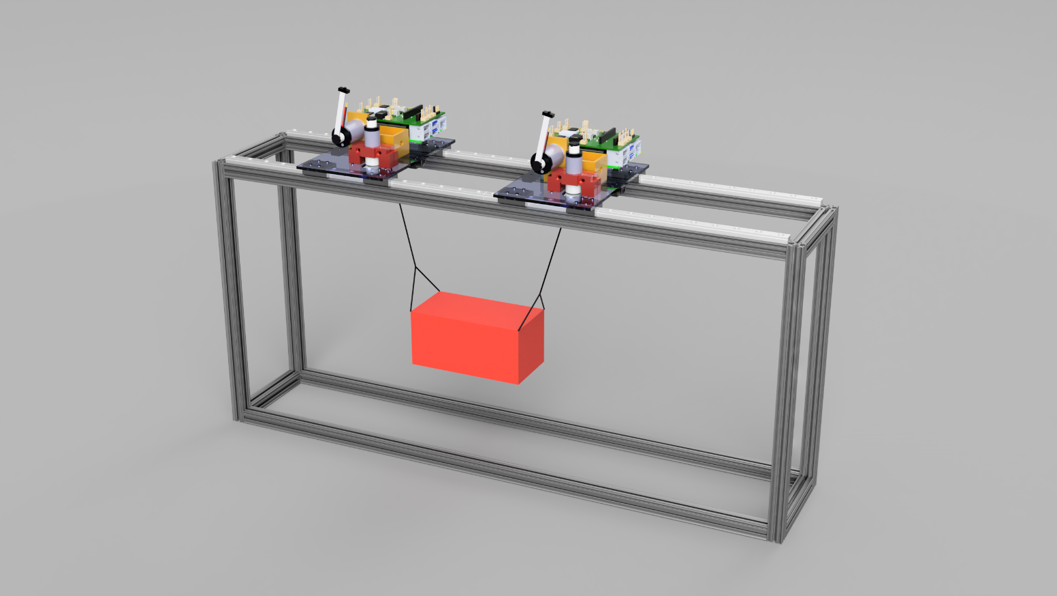
\includegraphics[scale=0.55]{Pictures/Veritas_demo_CAD.png}
	\end{center}
	\caption[Konstruktionsmodell des Doppelkransystems]
	{Konstruktionsmodell des Doppelkran-Demonstratorsystems ohne Verkabelung.}
	\label{fig:demonstrator_CAD}
\end{figure}

Das Demonstratorsystem besteht aus zwei Brückenkränen, die eine gemeinsame Last in der vertikalen Ebene anheben. Abbildung \ref{fig:demonstrator_CAD} stellt ein Modell des Aufbaus dar, das während des Konstruktionsprozesses entstanden ist. Die Kräne befinden sich auf zwei horizontalen Führungsschienen und verfügen jeweils über einen Raspberry Pi 4B\footnote{Spezifikationen: 8GB DDR4 RAM, 64-bit ARM64 SoC, 5.0 GHz WLAN, Bluetooth 5.0, BLE, Gigabit Ethernet; Betriebsystem: Ubuntu 20.04 \cite{RpiSpecs}} als Hauptrecheneinheit sowie einen STM32-Mikrocontroller\footnote{Spezifikationen: STM32F303K8 mit 32-bit Arm Cortex-M4, 64 kB Flash-Speicher, 12-bit ADCs \cite{STM32Specs}} für die Motoransteuerungen und Messungen. Beide Raspberry Pis können über eine LAN-Verbindung miteinander kommunizieren.

Die Kräne sind als Laufkatzen entlang der Schienen sowie Seilwinden darauf mit jeweils einem Gleichstrommotor aktuiert. Auf den STM32-Mikrocontrollern ist bereits eine unterlagerte Strom- beziehungsweise Kraftregelung für diese Motoren implementiert.
Messungen der Seillängen und Kranpositionen auf der Schiene erfolgen mittels Inkrementalgebern nach einem anfänglichen Kalibrierungsvorgang. Die Seilwinkel zur Horizontalen werden mittels mitschwingender Potentiometer bestimmt. Abbildung \ref{fig:demonstrator_real} zeigt eine Fotografie der realen Anordnung des Demonstrators.

\begin{figure}[ht]
	\begin{center}
		% hier keine Skalierung notwendig, wenn Datei schon mit passender figsize angelegt wurde:
		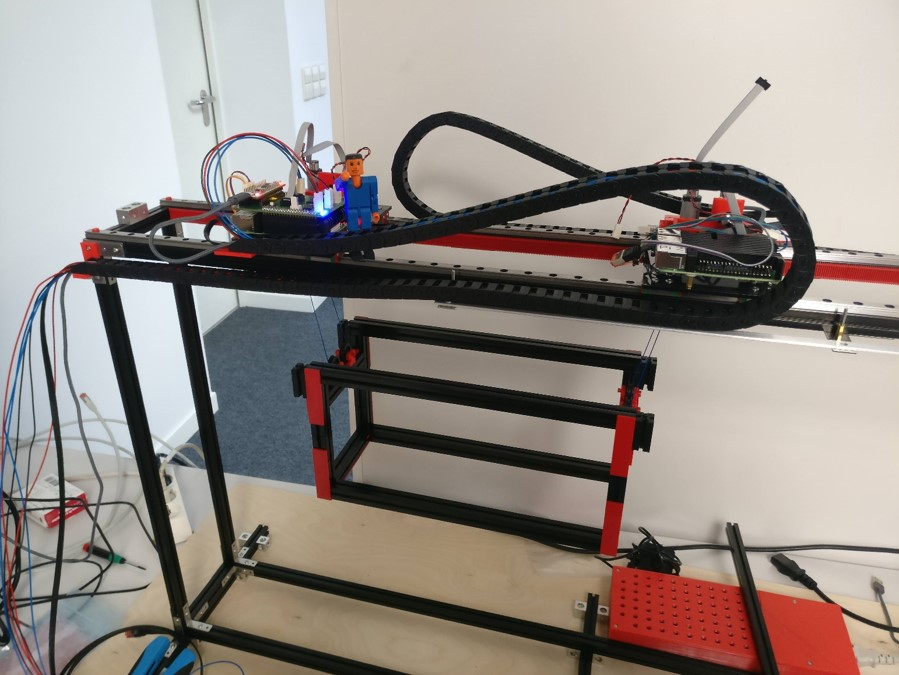
\includegraphics[scale=0.11]{Pictures/real_gantry.jpg}
	\end{center}
	\caption[Doppelkran-Demonstratorsystem mit Laufkatzen und Last]
	{Reale Anordnung des Doppelkran-Demonstratorsystems mit Laufkatzen und Last.}
	\label{fig:demonstrator_real}
\end{figure}

\section{Problembeschreibung und Zielsetzung}
Bei der Bewegung von Containern in Häfen ist ein ruckarmer und gegenüber der Horizontalen stabiler Transport notwendig. Ziel dieser Studienarbeit ist es deshalb,  bezüglich des vorhandenen Demonstratorsystems eine zentrale Referenzregelstrategie zu entwerfen. Damit soll unter Vorgabe von Sollposen eine Planung von Trajektorien der Last in der Ebene und Folgeregelung zur Überführung dieser zwischen verschiedenen Ruhelagen ermöglicht werden. Diese Überlegungen sollen auf Basis einer Modellierung des Krans als Mehrkörpersystems geschehen. 

\chapter{Analytische Modellbildung}

\section{Allgemeine Modellannahmen}

\textcolor{red}{In der folgenden Modellierung wird das Demonstratorsystem nur planar betrachtet, also die Bewegung aller Komponenten nur in der vertikalen Ebene berücksichtigt. Diese Annahme ist gerechtfertigt, weil die Laufkatzen nur entlang einer Achse verfahren können und die Lagerung bzw. Aufhängung der Last ein Schwingen dieser senkrecht zur vertikalen Ebene unterdrückt. Die Seile werden aufgrund ihrer geringen Dicke als masselos im Vergleich zu den Laufkatzen sowie der Last angenommen und nicht mit einem Trägheitsmoment versehen. Die Last wird trotz ihrer Aussparungen mit einer homogenen Masseverteilung modelliert. Für eine exakte Beschreibung wären Konstruktionsdaten oder eine Demontage mit Vermessung der Teilkomponenten notwendig. Zur Reduktion weiterer Komplexität wird auf die Abbildung dissipativer Kräfte im System verzichtet.}

\textcolor{red}{Die Modellbildung erfolgt in mehreren Stufen. Zunächst ist es möglich mittels der Lagrange-Gleichungen erster Art einen Einzelkran darzustellen, woraus ein gewöhnliches Differenzialgleichungssystem (DGL-System, engl. ODE system) folgt. Alternativ kann ein Ansatz mit Lagrange-Gleichungen zweiter Art gewählt werden, wodurch sich ein Differenzial-algebraisches Gleichungssystem (DAE-System, von engl. differential algebraic equations) ergibt. Ausgehend davon und aufgrund der geringen Komplexität der Terme des Einzelkrans, kann diese prinzipielle Methodik verifiziert werden und ein Transfer der Erkenntnisse auf die Modellierung des Doppelkransystems erfolgen.}

\textcolor{red}{Nun wird ein kurzer theoretischer Überblick zu beiden erwähnten Arten des Lagrange-Formalismus gegeben.}

\section{Modellierung mittels Lagrange-Formalismus}
Die Dynamik mechanischer Systeme lässt sich über Differenzialgleichungen, den sogenannten Lagrange-Gleichungen beschreiben. Dabei wird eine Menge aus $n$ auftretenden und zeitlich veränderlichen Koordinaten als Konfigurationskoordinaten oder Systemgrößen $\boldsymbol{\theta} = (\theta_1, ..., \theta_n)^T$ bezeichnet. Die zeitlichen Änderungsraten dieser werden im Vektor der (Konfigurations-)Geschwindigkeiten $\dot{\boldsymbol{\theta}}$ zusammengefasst. \textcolor{red}{Anfänglich wurde der Literatur \cite[S.10]{DissKnoll} folgend eine Unterteilung der Systemgrößen in ``aktive'' und ``passive'' Koordinaten vorgenommen. Im Verlauf dieser Arbeit ist bemerkt worden, dass die 
Aufgliederung $\boldsymbol{\theta} = (\mathbf{q}, \mathbf{p})^T$ in die direkt aktuierten Koordinaten $\mathbf{q}$ und nicht direkt aktuierten Koordinaten $\mathbf{p}$ eine treffendere Bezeichnung darstellt.}
\cite[S.7]{DissKnoll} 

Die kinetische Energie eines Systems wird im Folgenden durch die Funktion $T$ sowie die potentielle Energie durch $V$ beschrieben. Die Lagrange-Funktion kann damit folgendermaßen definiert werden:
\begin{equation}
L(\boldsymbol{\theta}, \dot{\boldsymbol{\theta}}) = T(\boldsymbol{\theta}, \dot{\boldsymbol{\theta}}) - V(\boldsymbol{\theta}).
\end{equation}

Eine stark automatisierte Durchführung dieses Formalismus ist unter Nutzung des Python-Pakets symbtools \cite{symbtools} möglich.

\subsection{Lagrange-Gleichungen erster Art}
\label{sec:Lagrange1_theory}

Mit den Lagrange-Gleichungen erster Art können Problemstellungen mit Zwangsbedingungen und -kräften dargestellt werden:
\begin{equation}
	\label{eq:lagrange1}
	\diff{}{t}\left(\partiell{L}{\dot{\theta}_i} \right) - \partiell{L}{\theta_i} = \tilde{Q}_i + Q_i, \quad i = 1, ..., n.
\end{equation}

Die sich auf die jeweilige Koordinate $\theta_i$ beziehende Stellkraft $Q_i = f_i - D_i$ entspricht der verallgemeinerten Kraft, welche sich aus der äußeren (Stell-)Kraft $f_i$ sowie internen Reibungskraft $D_i$ zusammensetzt \cite[S. 49]{Lagrange}.

Es können nun $m$ holonome Zwangsbedingungen $g_1(\boldsymbol{\theta}) = ... = g_m(\boldsymbol{\theta}) = 0$ eingeführt werden, aus denen die Zwangskraft $\tilde{Q}_i$ in Richtung der Koordinate $\theta_i$ folgt:
\begin{equation}
	\tilde{Q}_i = \sum_{j = 1}^m \lambda_j \textcolor{red}{\partiell{g_j}{\theta_i}}.
\end{equation}
In dieser Beziehung bezeichnet $\lambda_j$ den jeweiligen Lagrange-Multiplikator.

\subsection{Lagrange-Gleichungen zweiter Art}
\label{sec:Lagrange2_theory}
Die Lagrange-Gleichungen zweiter Art beschreiben bezüglich der Lagrange-Gleichungen erster Art den Spezialfall ohne Zwangsbedingungen, also $m = 0$. Zwangskräfte müssen dabei nicht explizit bestimmt werden. Die Bewegungsgleichungen können folgendermaßen aus der Lagrange-Funktion abgeleitet werden:
\begin{equation}
	\label{eq:lagrange2}
	\diff{}{t}\left(\partiell{L}{\dot{\theta}_i} \right) - \partiell{L}{\theta_i} = Q_i, \quad i = 1, ..., n.
\end{equation} 

Zur Bestimmung der Komponenten $Q_i$ der verallgemeinerten Kraft wird das Prinzip der virtuellen Arbeit herangezogen \cite{VirtualWork}:
\begin{equation}
	\delta W = \sum_{k=1}^l \mathbf{F}_k \cdot \frac{\partial \mathbf{r}_k}{\partial \theta_1} \delta \theta_1 +\ldots + \sum_{k=1}^l \mathbf{F}_k \cdot \frac{\partial \mathbf{r}_k}{\partial \theta_n} \delta \theta_n.
\end{equation}

Dabei entspricht $\mathbf{r_k}$ bei einem System von $l$ (massebehafteten) Teilchen dem Richtungsvektor zum $k$-ten Partikel, $\mathbf{F_k}$ der jeweils entlang dieses Richtungsvektors angewandten Stellkraft, $\delta \mathbf{r_{k}}$ der virtuellen Verschiebung des Partikels im Raum und $\delta \boldsymbol{\theta}_{i}$ der virtuellen Verschiebung der Koordinate $\theta_i$, welche der Beziehung
\begin{equation}
	\delta \mathbf{r_{k}} = \sum_{i = 1}^{n} \partiell{\mathbf{r_{k}}}{\theta_i} \delta \theta_i.
\end{equation}
genügt.

Die gesamte virtuelle Arbeit des Systems dieser Teilchen kann also ebenso durch
\begin{equation}
\label{eq:virtual_work}
\delta W = Q_1 \delta \theta_1 + \ldots + Q_n\delta \theta_n = \sum_{k=1}^{l}\delta \mathbf{r}_k^T \mathbf{F}_k
\end{equation}
dargestellt werden, wobei sich die Komponenten der verallgemeinerten Kraft zu
\begin{equation}
\label{eq:virtual_work_force}
Q_i = \sum_{k=1}^l \left(\frac {\partial \mathbf{r_k}} {\partial \theta_i} \right)^T \mathbf {F}_{k} = \partiell{\delta W}{\delta \theta_i} ,\quad i=1,\ldots, n 
\end{equation}
ergeben.
\section{Generierung und Simulation von DAE-Systemen}
DAE-Systeme sind ODE-Systeme, welche um algebraische Gleichungen (AGL, auch Nebenbedingungen) ergänzt werden. Diese Nebenbedingungen können zur Darstellung von Zwangsbedingungen der Lagrange-Gleichungen erster Art genutzt werden. DAE-Systeme lassen sich typischerweise in einer semi-expliziten Form darstellen:
	\begin{align}\label{eq:dae_std}
		\mathbf{\dot{x}} &= \mathbf{f}(\mathbf{x}, \mathbf{z}, \mathbf{u}, t) \\
		\mathbf{0} &= \mathbf{g}(\mathbf{x}, \mathbf{z}, t),
	\end{align}
wobei $\mathbf{x}$ dem Systemzustand, $\mathbf{z}$ den algebraischen Variablen (weitere Systemgrößen, die in den Systemgleichungen ohne Ableitung vorkommen), $\mathbf{u}$ dem Systemeingang sowie $t$ der Zeit entspricht. \cite[S.137]{JanschekSystementwurf}

Eine Möglichkeit zu Klassifikation von DAE-Systemen ist der differenzielle Index $i_\mathrm{d}$. Dieser entspricht der minimalen Anzahl an Differenziationen $\frac{d}{dt}$ der AGL $\mathbf{g}$ (Zwangsbedingungen), damit unter Einbeziehung der DGL ein explizites DGL-System aus dem DAE-System entsteht. Ein gewöhnliches DGL-System besitzt also den differenziellen Index $i_\mathrm{d} = 0$. Die Differenziation der AGL mit dem Resultat eines DAE-Systems mit kleinerem Index wird als Indexreduktion bezeichnet. \cite[S.139]{JanschekSystementwurf}

Für die Simulation von DAE-Systemen ist die numerische Integration dieser Gleichungssysteme notwendig. Die in dieser Arbeit untersuchten mechanischen Systeme sind solche mit starrer Kopplung als Zwangsbedingungen vom Index $i_\mathrm{d} = 3$ und können für den Zustandsvektor $\mathbf{x} = (\boldsymbol{\theta}, \dot{\boldsymbol{\theta}})^T$ über folgende Bewegungsgleichungen mittels der Matrizen $\mathbf{M}$, $\mathbf{C}$, $\mathbf{K}$, $\mathbf{G}$ und $\mathbf{B}$ beschrieben werden:
\begin{subequations}
\label{eq:implicit_mechanical_system}
\begin{align}
	\mathbf{0} &= \mathbf{M}(\boldsymbol{\theta}) \ddot{\boldsymbol{\theta}} + \mathbf{C}(\boldsymbol{\theta}, \dot{\boldsymbol{\theta}}) + \mathbf{K}(\boldsymbol{\theta}, \dot{\boldsymbol{\theta}}) + \mathbf{G}(\boldsymbol{\theta}) \mathbf{z} - \mathbf{B}(\boldsymbol{\theta}) \mathbf{u}\\
	\mathbf{0} &= \mathbf{g}(\boldsymbol{\theta}).
\end{align}
\end{subequations}
\cite[S.240]{JanschekSystementwurf}

Zur Integration davon gibt es verschiedene Möglichkeiten \cite[Kap. 8]{ModSimSkript}: 
\begin{itemize}
\item  Indexreduktion auf Index $i_\mathrm{d} = 2$ und anschließende Integration über ein implizites\footnote{Auf der linken und rechten Seite der zu integrierenden Gleichungen sind die gesuchten Näherungswerte von $\mathbf{x}(t_{i+1})$ an der Stelle $t_{i+1}$ enthalten.} Verfahren
\item Indexreduktion auf Index $i_\mathrm{d} = 1$ und anschließende Integration über ein explizites\footnote{Zur Berechnung des Näherungswertes von $\mathbf{x}(t_{i+1})$ an der Stelle $t_{i+1}$ wird einzig der zuletzt berechnete Näherungswert von $\mathbf{x}(t_{i})$ an der Stelle $t_{i}$ benötigt.} Verfahren mit AGL-Löser oder ein implizites Verfahren
\item Indexreduktion auf Index  $i_\mathrm{d} = 0$ und anschließende Integration über ein explizites oder implizites Verfahren.
\end{itemize}
Die im Python-Paket symbtools \cite{symbtools} enthaltene Bibliothek modeltools führt die Reduktion von Index-3-Systemen auf Index-1-Systeme durch. Zur numerischen Berechnung kann daraufhin der Solver ODASSL des Python-Pakets assimulo \cite{assimulo} verwendet werden.

Zur Erfüllung der AGL zu Simulationsbeginn müssen konsistente Anfangswerte $\mathbf{x}(0)$ und $\mathbf{z}(0)$ bestimmt werden. Bei DAE-Systemen mit Index $i_\mathrm{d} \geq 2$  kann $\mathbf{x}(0)$ nicht mehr frei gewählt werden, da $\mathbf{z}(0)$ nicht mehr allein aus AGL bestimmbar ist. Es ist notwendig, zusätzliche algebraische Bedingungen an $\mathbf{x}$ und $\mathbf{z}$ aus den DGL abzuleiten. Die Bibliothek modeltools berechnet konsistente Anfangswerte mit der Funktion \texttt{calc\_consistent\_init\_vals}. Falls es andernfalls zu inkonsistenten Anfangswerten kommt, folgen daraus Simulationsfehler in den ersten Schritten oder sogar vollständig falsche Ergebnisse. \cite[S.207]{JanschekSystementwurf}

\section{Analytisches Modell des Einzelkrans}
\label{sec:single_crane}
Eine Implementierung der in diesem Abschnitt durchgeführten Überlegungen ist unter \cite[flatness\_notebooks/ODE\_flatness\_analysis\_single\_crane.ipynb]{SAGithub} zu finden.

Mittels der Lagrange-Gleichungen zweiter Art wird in diesem Abschnitt ein ODE-Modell des Einzelkrans erzeugt. Dabei wird entsprechend der Erläuterungen aus Abschnitt \ref{sec:Lagrange2_theory} vorgegangen. Diese Modellierung hat gegenüber den Lagrange-Gleichungen erster Art  den Vorteil, dass durch die generalisierte Kraft $\mathbf{Q}$ gerade die Stellkraft im Seil gut abgebildet werden kann sowie eine Vielzahl verschiedener Integrationsverfahren für eine effiziente Lösung des ODE-Systems nutzbar ist. Abbildung \ref{fig:single_crane_diagram} zeigt die Konfiguration des Einzelkransystems.

\begin{figure}[ht]
	\begin{center}
		% hier keine Skalierung notwendig, wenn Datei schon mit passender figsize angelegt wurde:
		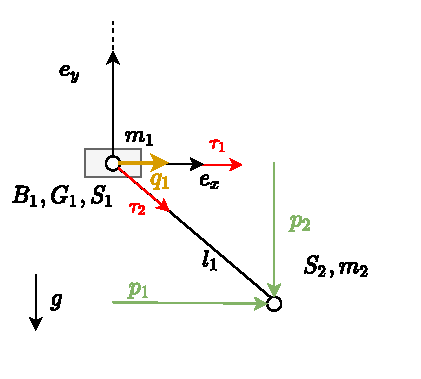
\includegraphics[scale=1]{Pictures/ODE_flatness_analysis_single_crane_diagram}
	\end{center}
	\caption[Planare Geometrie des Einzelkransystems]
	{Planare Geometrie des Einzelkransystems mit Systemgrößen, Systemparametern und Kräften.}
	\label{fig:single_crane_diagram}
\end{figure}

Als direkt aktuierte Koordinate wird nur die $x$-Verschiebung $q_1$ der Laufkatzenposition ($\mathbf{B}_1 = \mathbf{G}_1 = \mathbf{S}_1$) ausgewählt, als nicht direkt aktuierte Koordinaten die $x$- und $y$-Auslenkungen $(p_1, p_2)$ der Last $\mathbf{S}_2$ aus dem Ursprung. Die variable Seillänge wird mit $l_1$ bezeichnet, die durch die Koordinaten auch mittels
\begin{equation}
	l_1 = \sqrt{(p_1 - q_1)^2 + p_2^2}
\end{equation}
ausgedrückt werden kann.

Die Position der beiden Massenschwerpunkte kann somit wie folgt durch die Koordinaten beschrieben werden:
\begin{equation}
	\mathbf{S}_1 =
	\begin{pmatrix}
		q_1 \\
		0
	\end{pmatrix}, 
	\quad
	\mathbf{S}_2 =
	\begin{pmatrix}
		p_1 \\
		p_2
	\end{pmatrix}.
\end{equation}

Damit ist es möglich die kinetische und potentielle Energie des Systems zu formulieren:
\begin{align}
	T &= \frac{m_1}{2} \dot{\mathbf{S}}_1^T \dot{\mathbf{S}}_1 + \frac{m_2}{2} \dot{\mathbf{S}}_2^T \dot{\mathbf{S}}_2 = \frac{m_{1} \dot{q}_{1}^{2}}{2} + \frac{m_{2} \dot{p}_{1}^{2}}{2} + \frac{m_{2} \dot{p}_{2}^{2}}{2} \\
	V &= m_2 g \ \mathbf{S}_2^T \mathbf{e}_y = m_{2} g p_{2}.
\end{align}

Die Systemgleichungen können durch die Lagrange-Gleichungen zweiter Art \eqref{eq:lagrange2} zunächst in Abhängigkeit der Komponenten der generalisierten Kraft $Q_i$ bestimmt werden:
\begin{subequations}
	\label{eq:single_crane_sys_w_Q}
	\begin{align}
		- Q_{1} + m_{2} \ddot{p}_{1} &= 0\\
		- Q_{2} + g m_{2} + m_{2} \ddot{p}_{2} &= 0\\
		- Q_{3} + m_{1} \ddot{q}_{1} &= 0.
	\end{align}
\end{subequations}


Die Eingangskomponenten $\tau_1$, $\tau_2$ des Systems entsprechen den unterlagert geregelten Kräften der Motoren der Laufkatze bzw. der Seilwinde. Sie können über Stellkräfte vektoriell dargestellt werden:
\begin{equation}
	\mathbf{F}_1 =
	\left(\begin{matrix}
		\tau_{1} \\
		0
	\end{matrix}\right), \quad
	\mathbf{F}_2 =
	\left(\begin{matrix}
		\frac{\tau_{2} \left(p_{1} - q_{1}\right)}{l_{1}}\\
		\frac{p_{2} \tau_{2}}{l_{1}}
	\end{matrix}\right).
\end{equation}

Durch die Anwendung des Prinzips der virtuellen Arbeit nach Gleichung \eqref{eq:virtual_work} und \eqref{eq:virtual_work_force} ist es möglich, die generalisierte Kraft durch diese Stellkräfte bzw. den Systemeingang auszudrücken:
\begin{equation}
	\mathbf{Q}=
	\left(\begin{matrix}
		\frac{\tau_{2} \left(p_{1} - q_{1}\right)}{l_{1}}\\
		\frac{p_{2} \tau_{2}}{l_{1}}\\
		\tau_{1} - \frac{\tau_{2} \left(p_{1} - q_{1}\right)}{l_{1}}
	\end{matrix}\right).
\end{equation}

Durch einsetzen dieser generalisierten Kraft in die Gleichungen \eqref{eq:single_crane_sys_w_Q} lässt sich ein abschließender Satz an Systemgleichungen des Einzelkrans bilden:
\begin{subequations}
	\begin{align}
		m_{2} \ddot{p}_{1} - \frac{\tau_{2} \left(p_{1} - q_{1}\right)}{l_{1}} &= 0 \label{single_flat_syseq1}\\
		g m_{2} + m_{2} \ddot{p}_{2} - \frac{p_{2} \tau_{2}}{l_{1}} &= 0\label{single_flat_syseq2}\\
		m_{1} \ddot{q}_{1} - \tau_{1} + \frac{\tau_{2} \left(p_{1} - q_{1}\right)}{l_{1}} &= 0\label{single_flat_syseq3}.
	\end{align}
\end{subequations}


\section{Analytisches Modell des Doppelkrans}
\textcolor{red}{Aufbauend auf der Modellierung eines Einzelkrans wird in diesem Abschnitt eine Erweiterung des Systems auf ein Doppelkransystem in Analogie zum realen Demonstrator vorgenommen. Aufgrund der an beiden Laufkatzen befestigten Last liegt zunächst alternativ zum vorherigen Vorgehen die Nutzung der Lagrange-Gleichungen erster Art nahe. Bei dieser wird mittels algebraischer Zwangsbedingungen ein DAE-System erzeugt. Allerdings ist dabei die Beschreinung der Aktuierung der Seilwinden anspruchsvoller, da bereits für eine konstante Seillänge die bei der Katzfahrt auftretenden dynamischen Seilkräfte kompensiert werden müssen, ohne dass es dafür eine explizite resultierende Gesamtkraft gibt, die zu Null gesetzt werden kann. Beim realen Demonstrator sperrt ein Schneckengetriebe der Seilwinde im stromfreien Fall die Hubaktuierung. Auch bei einem Doppelkransystem ist wieder eine Modellierung mit den Lagrange-Gleichungen zweiter Art möglich.}

\subsection{Ansatz über ein DAE-System (Lagrange 1)}
Eine Implementierung der in diesem Abschnitt durchgeführten Überlegungen ist unter \cite[double\_crane\_notebooks/DAE\_double\_crane\_cartesian.ipynb]{SAGithub} zu finden.

Mittels der Lagrange-Gleichungen erster Art wird im Folgenden ein DAE-Modell des Doppelkrans erzeugt. Dabei wird entsprechend Abschnitt \ref{sec:Lagrange1_theory} vorgegangen. Schließlich ergibt sich hierbei ein komplexerer Satz an Systemgleichungen, die typischerweise weniger effizient zu simulieren sind als bei einem ODE-System. Daher wird dieser Ansatz in weiteren Kapiteln nicht weiter verfolgt. Eine Dokumentation dieser Modellierung ist trotzdem sinnvoll. Durch die Einprägung von Zwangsbedingungen kann die kinematische Kette\footnote{Bezeichnung, die auf den Vergleich des Systems mit einem Viergelenk aus der Literatur abzielt, durch die gemeinsame Last wird die Kette "geschlossen"} wegen der gemeinsamen Last intuitiv abgebildet werden. Es wird zunächst einzig eine horizontale Aktuierung der Laufkatzen durch den Eingang $\boldsymbol{\tau} = (\tau_{1}, \tau_{2})^T$ betrachtet. Für eine effiziente Simulation mit aktuierten Seilwinden, welche für diesen Ansatz nicht mehr im Rahmen dieser Studienarbeit durchgeführt wird, wäre gerade bei konstanten Seillängen eine Umformulierung des Problems mit den Seillängen als Stellgröße sinnvoll. \textcolor{red}{(Quelle: Buch von Rudolf S.21 -> Nextcloud Flachheit/fotos ???)} Abbildung \ref{fig:DAE_double_crane_diagram} zeigt die Konfiguration dieses Doppelkransystems.

\begin{figure}[ht]
	\begin{center}
		% hier keine Skalierung notwendig, wenn Datei schon mit passender figsize angelegt wurde:
		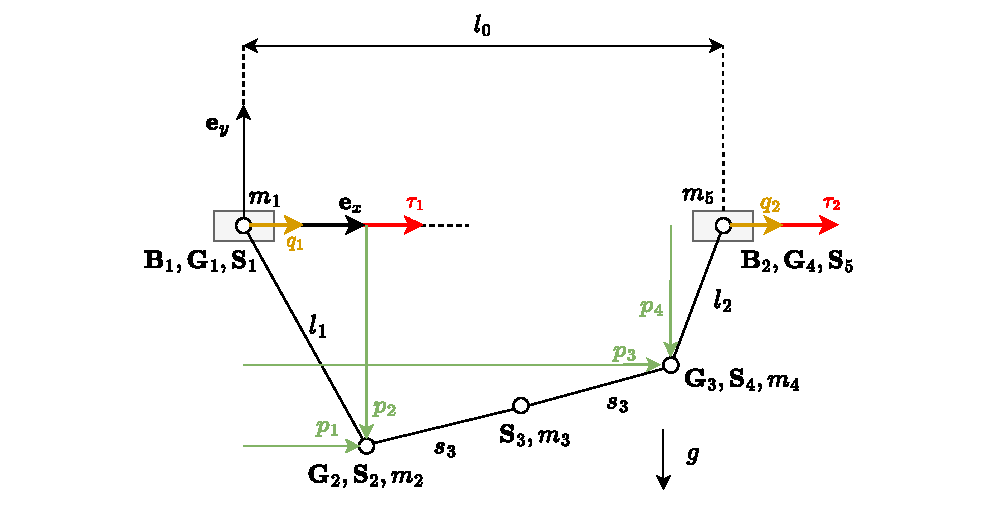
\includegraphics[scale=1]{Pictures/DAE_double_crane_cartesian_diagram.pdf}
	\end{center}
	\caption[Planare Geometrie des Doppellkransystems im DAE-Modell]
	{Planare Geometrie des Doppellkransystems im DAE-Modell mit Systemgrößen, Systemparametern und Kräften.}
	\label{fig:DAE_double_crane_diagram}
\end{figure}

Als direkt aktuierte Koordinate werden nur die $x$-Verschiebungen $q_1$ und $q_2$ der Laufkatzenpositionen ($\mathbf{B}_1 = \mathbf{G}_1 = \mathbf{S}_1$, $\mathbf{B}_2 = \mathbf{G}_4 = \mathbf{S}_5$) ausgewählt, als nicht direkt aktuierte Koordinaten die absolute Position $(p_1, p_2)$ des Gelenks $\mathbf{G}_2 (= \mathbf{S}_2)$ sowie $(p_3, p_4)$ des Gelenks $\mathbf{G}_3 (=\mathbf{S}_4)$. 

Für konstante Seillängen können folgende Zwangsbedingungen formuliert werden:
\begin{align}
	l_{1} - \sqrt{p_{2}^{2} + \left(p_{1} - q_{1}\right)^{2}} &= 0\\
	l_{2} - \sqrt{p_{4}^{2} + \left(- l_{0} + p_{3} - q_{2}\right)^{2}} &= 0.	
\end{align}

Die konstante Lastlänge wird durch
\begin{equation}
	2 s_{3} = \sqrt{\left(p_{1} - p_{3}\right)^{2} + \left(p_{2} - p_{4}\right)^{2}}
\end{equation}
ausgedrückt.

Die Position der Massenschwerpunkte und Gelenke kann somit wie folgt durch die Koordinaten beschrieben werden:
\begin{align}
	\mathbf{S}_1 =
	\begin{pmatrix}
		q_1 \\
		0
	\end{pmatrix}, 
	\
	\mathbf{S}_2 =
	\begin{pmatrix}
		p_1 \\
		p_2
	\end{pmatrix},
	\
	\mathbf{S}_3 =
	\frac{1}{2}(\mathbf{S}_2 + \mathbf{S}_4) =
	\frac{1}{2}
	\begin{pmatrix}
		p_1 + p_3 \\
		p_2 + p_4
	\end{pmatrix},
	\nonumber \\
	\mathbf{S}_4 =
	\left(\begin{matrix}
		p_3 \\
		p_4
	\end{matrix}\right),
	\
	\mathbf{S}_5 =
	\left(\begin{matrix}
		l_0 + q_2 \\
		0
	\end{matrix}\right).
\end{align}

Es ist notwendig, dass alle abgeleiteten Koordinaten in der kinetischen Energie $T$ vorhanden sind, damit die Massenmatrix $\mathbf{M}(\boldsymbol{\theta})$ in Gleichung \eqref{eq:implicit_mechanical_system} regulär ist \cite[${\text{S. 7}}$]{DissKnoll}. Dies wäre bei einer Modellierung der Last mit homogener Masseverteilung und homogenem Trägheitsmoment nicht der Fall. Deshalb wird die Last durch ein System aus drei Massen ($m_2$, $m_3$, $m_4$) beschrieben, das sich unter Einhaltung der folgenden Zusammenhänge simulativ äquivalent verhält:
\begin{align}
	m_{\mathrm{ges}} &= m_2 + m_3 + m_4\\
	m_2 &= m_4\\
	J &= m_2 s_3^2 + m_4 s_3^2 = 2 m_2 s_3^2\\
	\Rightarrow m_2 &= m_4 = \frac{J}{2 s_3^2} \\
	\Rightarrow m_3 &= m_{\mathrm{ges}} - m_2 -m_4.
\end{align}

Die Größen $m_{\mathrm{ges}}$ und $J$ beziehen sich auf die in Abschnitt \ref{sec:SysIdent} identifizierten Systemparameter, die so auch bei der Modellbildung des Doppelkrans als ODE-System genutzt wurden.

Somit ist es möglich, die kinetische und potentielle Energie des Systems zu formulieren:
\begin{align}
	T &= \frac{m_1}{2} \dot{\mathbf{S}}_1^T \dot{\mathbf{S}}_1 + \frac{m_2}{2} \dot{\mathbf{S}}_2^T \dot{\mathbf{S}}_2 + \frac{m_3}{2} \dot{\mathbf{S}}_3^T \dot{\mathbf{S}}_3 + \frac{m_4}{2} \dot{\mathbf{S}}_4^T \dot{\mathbf{S}}_4 + \frac{m_5}{2} \dot{\mathbf{S}}_5^T \dot{\mathbf{S}}_5 \nonumber \\  
	&= \frac{m_{1} \dot{q}_{1}^{2}}{2} + \frac{m_{2} \dot{p}_{1}^{2}}{2} + \frac{m_{2} \dot{p}_{2}^{2}}{2} + \frac{m_{3} \cdot 0.25 \left(\dot{p}_{1} + \dot{p}_{3}\right)^{2}}{2} + \frac{m_{3} \cdot 0.25 \left(\dot{p}_{2} + \dot{p}_{4}\right)^{2}}{2} \nonumber \\
	&+ \frac{m_{4} \dot{p}_{3}^{2}}{2} + \frac{m_{4} \dot{p}_{4}^{2}}{2} + \frac{m_{5} \dot{q}_{2}^{2}}{2} \\
	V &= (m_2 \ g \ \mathbf{S}_2^T + m_3 \ g \ \mathbf{S}_3^T + m_4 \ g \ \mathbf{S}_4^T) \mathbf{e}_y \nonumber \\ &= g \left(m_{2} p_{2} + m_{3} \left(0.5 p_{2} + 0.5 p_{4}\right) + m_{4} p_{4}\right).
\end{align}

Unter Nutzung der Lagrange-Multiplikatoren $\lambda_j$ ist es mittels der Lagrange-Gleichungen zweiter Art \eqref{eq:lagrange1} möglich die Systemgleichungen auszudrücken als:
\begin{subequations}
	\begin{flalign}
		&- \frac{\lambda_{1} p_{1}}{\sqrt{p_{2}^{2} + \left(p_{1} - q_{1}\right)^{2}}} + \frac{\lambda_{1} q_{1}}{\sqrt{p_{2}^{2} + \left(p_{1} - q_{1}\right)^{2}}} - \frac{\lambda_{2} p_{1}}{\sqrt{\left(p_{1} - p_{3}\right)^{2} + \left(p_{2} - p_{4}\right)^{2}}} \nonumber \\
		&+ \frac{\lambda_{2} p_{3}}{\sqrt{\left(p_{1} - p_{3}\right)^{2} + \left(p_{2} - p_{4}\right)^{2}}} + m_{2} \ddot{p}_{1} + 0.25 m_{3} \ddot{p}_{1} + 0.25 m_{3} \ddot{p}_{3} = 0\\
		&g m_{2} + 0.5 g m_{3} - \frac{\lambda_{1} p_{2}}{\sqrt{p_{2}^{2} + \left(p_{1} - q_{1}\right)^{2}}} - \frac{\lambda_{2} p_{2} + \lambda_{2} p_{4}}{\sqrt{\left(p_{1} - p_{3}\right)^{2} + \left(p_{2} - p_{4}\right)^{2}}} \nonumber \\
		&+ m_{2} \ddot{p}_{2} + 0.25 m_{3} \ddot{p}_{2} + 0.25 m_{3} \ddot{p}_{4} = 0\\
		&\frac{\lambda_{2} \left(p_{1} - p_{3}\right)}{\sqrt{\left(p_{1} - p_{3}\right)^{2} + \left(p_{2} - p_{4}\right)^{2}}} + \frac{\lambda_{3} \left(l_{0} - p_{3} + q_{2}\right)}{\sqrt{p_{4}^{2} + \left(l_{0} - p_{3} + q_{2}\right)^{2}}} \noindent \\
		&+ \frac{m_{3} \left(0.5 \ddot{p}_{1} + 0.5 \ddot{p}_{3}\right)}{2} + m_{4} \ddot{p}_{3} = 0\\
		&0.5 g m_{3} + g m_{4} + \frac{\lambda_{2} p_{2}}{\sqrt{\left(p_{1} - p_{3}\right)^{2} + \left(p_{2} - p_{4}\right)^{2}}} - \frac{\lambda_{2} p_{4}}{\sqrt{\left(p_{1} - p_{3}\right)^{2} + \left(p_{2} - p_{4}\right)^{2}}} \nonumber \\ 
		&- \frac{\lambda_{3} p_{4}}{\sqrt{p_{4}^{2} + \left(l_{0} - p_{3} + q_{2}\right)^{2}}} + 0.25 m_{3} \ddot{p}_{2} + 0.25 m_{3} \ddot{p}_{4} + m_{4} \ddot{p}_{4} = 0\\
		&\frac{\lambda_{1} \left(p_{1} - q_{1}\right) + \sqrt{p_{2}^{2} + \left(p_{1} - q_{1}\right)^{2}} \left(m_{1} \ddot{q}_{1} - \tau_{1}\right)}{\sqrt{p_{2}^{2} + \left(p_{1} - q_{1}\right)^{2}}} = 0\\
		&\frac{- \lambda_{3} \left(l_{0} - p_{3} + q_{2}\right) + \sqrt{p_{4}^{2} + \left(l_{0} - p_{3} + q_{2}\right)^{2}} \left(m_{5} \ddot{q}_{2} - \tau_{2}\right)}{\sqrt{p_{4}^{2} + \left(l_{0} - p_{3} + q_{2}\right)^{2}}} = 0.
	\end{flalign}
\end{subequations}

\subsection{Ansatz über ein ODE-System (Lagrange 2)}
\label{subsec:double_crane_lagrange2}
Eine Implementierung der in diesem Abschnitt durchgeführten Überlegungen ist unter \cite[flatness\_notebooks/ODE\_flatness\_analysis.ipynb]{SAGithub} zu finden.

Mittels der Lagrange-Gleichungen zweiter Art wird im Folgenden ein ODE-Modell des Doppelkrans erzeugt. Dabei wird entsprechend Abschnitt \ref{sec:Lagrange2_theory} vorgegangen. Abbildung \ref{fig:double_crane_diagram} zeigt die Konfiguration dieses Doppelkransystems.

\begin{figure}[ht]
	\begin{center}
		% hier keine Skalierung notwendig, wenn Datei schon mit passender figsize angelegt wurde:
		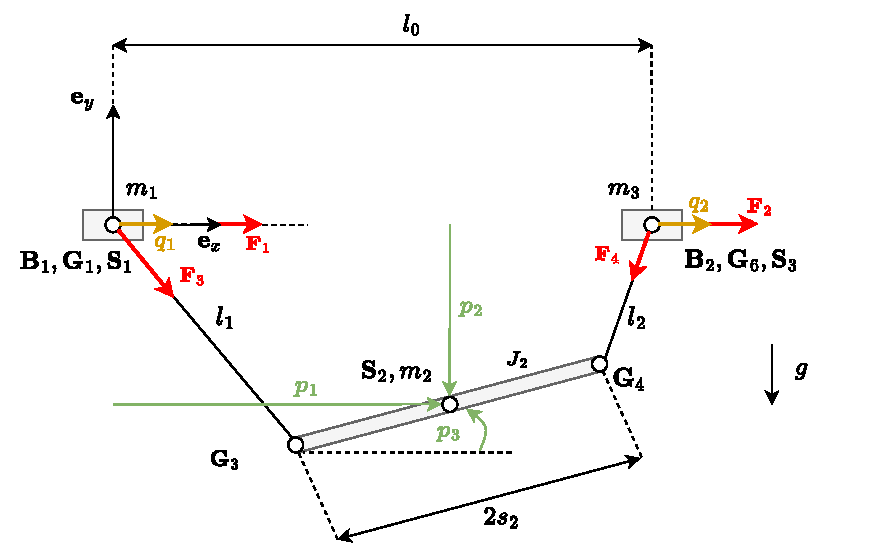
\includegraphics[scale=1]{Pictures/ODE_flatness_analysis_double_crane_diagram}
	\end{center}
	\caption[Planare Geometrie des Doppellkransystems im ODE-Modell]
	{Planare Geometrie des Doppellkransystems im ODE-Modell mit Systemgrößen, Systemparametern und Kräften.}
	\label{fig:double_crane_diagram}
\end{figure}


Als direkt aktuierte Koordinate werden zunächst nur die $x$-Verschiebungen $q_1$ und $q_2$ der Laufkatzenpositionen ($\mathbf{B}_1 = \mathbf{G}_1 = \mathbf{S}_1$, $\mathbf{B}_2 = \mathbf{G}_6 = \mathbf{S}_3$) ausgewählt, als nicht direkt aktuierte Koordinaten die absolute Position $(p_1, p_2)$ des Lastschwerpunkts ($\mathbf{S}_2$) sowie die Orientierung der Last $p_3$ gegenüber der Horizontalen. Die variable Seillänge wird mit $l_1$ sowie $l_2$ bezeichnet, die durch die Koordinaten auch mittels
\begin{align}
l_1 &= \sqrt{\left(p_{2} - s_{2} \sin{\left(p_{3} \right)}\right)^{2} + \left(p_{1} - q_{1} - s_{2} \cos{\left(p_{3} \right)}\right)^{2}} \\
l_2 &= \sqrt{\left(p_{2} + s_{2} \sin{\left(p_{3} \right)}\right)^{2} + \left(- l_{0} + p_{1} - q_{2} + s_{2} \cos{\left(p_{3} \right)}\right)^{2}}
\end{align}
ausgedrückt werden kann.

Die Position der Massenschwerpunkte und Gelenke kann somit wie folgt durch die Koordinaten beschrieben werden:
\begin{equation}
\begin{smallmatrix}
\mathbf{S}_1 =
\begin{pmatrix}
q_1 \\
0
\end{pmatrix}, 
\
\mathbf{S}_2 =
\begin{pmatrix}
p_1 \\
p_2
\end{pmatrix},
\
\mathbf{S}_3 =
\begin{pmatrix}
l_0 + q_2 \\
0
\end{pmatrix},
\
\mathbf{G}_3 =
\left(\begin{matrix}
p_{1} - s_{2} \cos{\left(p_{3} \right)}\\
p_{2} - s_{2} \sin{\left(p_{3} \right)}
\end{matrix}\right),
\
\mathbf{G}_4 =
\left(\begin{matrix}
p_{1} + s_{2} \cos{\left(p_{3} \right)}\\
p_{2} + s_{2} \sin{\left(p_{3} \right)}
\end{matrix}\right)
\end{smallmatrix}.
\end{equation}

Damit ist es möglich, die kinetische und potentielle Energie des Systems zu formulieren:
\begin{align}
T &= \frac{m_1}{2} \dot{\mathbf{S}}_1^T \dot{\mathbf{S}}_1 + \frac{m_2}{2} \dot{\mathbf{S}}_2^T \dot{\mathbf{S}}_2 + \frac{J_2}{2} \dot{p}_3^2 + \frac{m_3}{2} \dot{\mathbf{S}}_3^T \dot{\mathbf{S}}_3 \nonumber \\  
&= \frac{J_{2} \dot{p}_{3}^{2}}{2} + \frac{m_{1} \dot{q}_{1}^{2}}{2} + \frac{m_{2} \dot{p}_{1}^{2}}{2} + \frac{m_{2} \dot{p}_{2}^{2}}{2} + \frac{m_{3} \dot{q}_{2}^{2}}{2} \\
V &= m_2 g \ \mathbf{S}_2^T \mathbf{e}_y = m_{2} g p_{2}.
\end{align}

Die Systemgleichungen können durch die Lagrange-Gleichungen zweiter Art \eqref{eq:lagrange2} zunächst in Abhängigkeit der Komponenten der generalisierten Kraft $Q_i$ bestimmt werden:
\begin{subequations}
	\label{eq:double_crane_ODE_w_Q}
	\begin{align}
	- Q_{1} + m_{2} \ddot{p}_{1} &= 0\\
	- Q_{2} + g m_{2} + m_{2} \ddot{p}_{2} &= 0\\
	J_{2} \ddot{p}_{3} - Q_{3} &= 0\\
	- Q_{4} + m_{1} \ddot{q}_{1} &= 0\\
	- Q_{5} + m_{3} \ddot{q}_{2} &= 0.
	\end{align}
\end{subequations}

Über die Komponenten des Systemeingangs $\boldsymbol{\tau}$ und normierte Richtungsvektoren der Führungsschiene bzw. der Seile können die vektoriellen Stellkräfte dargestellt werden:
\begin{equation}
\begin{smallmatrix}
\mathbf{F}_1 =
\left(\begin{matrix}
\tau_{1} \\
0
\end{matrix}\right), \
\mathbf{F}_2 =
\left(\begin{matrix}
\tau_{2} \\
0
\end{matrix}\right), \
\mathbf{F}_3 =
\left(\begin{matrix}
\frac{\tau_{3} \left(p_{1} - q_{1} - s_{2} \cos{\left(p_{3} \right)}\right)}{l_{1}}\\
\frac{\tau_{3} \left(p_{2} - s_{2} \sin{\left(p_{3} \right)}\right)}{l_{1}}
\end{matrix}\right), \
\mathbf{F}_4 =
\left(\begin{matrix}
\frac{\tau_{4} \left(- l_{0} + p_{1} - q_{2} + s_{2} \cos{\left(p_{3} \right)}\right)}{l_{2}}\\
\frac{\tau_{4} \left(p_{2} + s_{2} \sin{\left(p_{3} \right)}\right)}{l_{2}}
\end{matrix}\right)
\end{smallmatrix}.
\end{equation}

Durch die Anwendung des Prinzips der virtuellen Arbeit ist es möglich, die generalisierte Kraft durch diese Stellkräfte bzw. den Systemeingang auszudrücken (Abkürzungen $\mathrm{s}_x := \sin{x}$ und $\mathrm{c}_x := \cos{x}$):
\begin{equation}
\mathbf{Q}=
\left(\begin{smallmatrix}
\frac{\tau_{4} \left(- l_{0} + p_{1} - q_{2} + s_{2} \mathrm{c}_{p_{3}}\right)}{l_{2}} + \frac{\tau_{3} \left(p_{1} - q_{1} - s_{2} \mathrm{c}_{p_{3}}\right)}{l_{1}}\\
\frac{\tau_{4} \left(p_{2} + s_{2} \mathrm{s}_{p_{3}}\right)}{l_{2}} + \frac{\tau_{3} \left(p_{2} - s_{2} \mathrm{s}_{p_{3}}\right)}{l_{1}}\\
\frac{s_{2} \tau_{4} \left(p_{2} + s_{2} \mathrm{s}_{p_{3}}\right) \mathrm{c}_{p_{3} }}{l_{2}} - \frac{s_{2} \tau_{4} \left(- l_{0} + p_{1} - q_{2} + s_{2} \mathrm{c}_{p_{3} }\right) \mathrm{s}_{p_{3}}}{l_{2}} - \frac{s_{2} \tau_{3} \left(p_{2} - s_{2} \mathrm{s}_{p_{3}}\right) \mathrm{c}_{p_{3}}}{l_{1}} + \frac{s_{2} \tau_{3} \left(p_{1} - q_{1} - s_{2} \mathrm{c}_{p_{3}}\right) \mathrm{s}_{p_{3}}}{l_{1}}\\
\tau_{1} - \frac{\tau_{3} \left(p_{1} - q_{1} - s_{2} \mathrm{c}_{p_{3} }\right)}{l_{1}}\\
\tau_{2} - \frac{\tau_{4} \left(- l_{0} + p_{1} - q_{2} + s_{2} \mathrm{c}_{p_{3} }\right)}{l_{2}}
\end{smallmatrix}\right).
\end{equation}

Durch Einsetzen dieser generalisierten Kraft in die Gleichungen \eqref{eq:double_crane_ODE_w_Q} lässt sich ein abschließender Satz an Systemgleichungen des Doppelkrans bilden:
\begin{subequations}
	\begin{flalign}
	&m_{2} \ddot{p}_{1} - \frac{\tau_{4} \left(- l_{0} + p_{1} - q_{2} + s_{2} \cos{\left(p_{3} \right)}\right)}{l_{2}} - \frac{\tau_{3} \left(p_{1} - q_{1} - s_{2} \cos{\left(p_{3} \right)}\right)}{l_{1}} = 0 \label{double_flat_syseq1}\\
	&g m_{2} + m_{2} \ddot{p}_{2} - \frac{\tau_{4} \left(p_{2} + s_{2} \sin{\left(p_{3} \right)}\right)}{l_{2}} - \frac{\tau_{3} \left(p_{2} s_{2} \sin{\left(p_{3} \right)}\right)}{l_{1}} = 0 \label{double_flat_syseq2}\\
	&J_{2} \ddot{p}_{3} - \frac{s_{2} \tau_{4} \left(p_{2} + s_{2} \sin{\left(p_{3} \right)}\right) \cos{\left(p_{3} \right)}}{l_{2}} + \frac{s_{2} \tau_{4} \left(- l_{0} + p_{1} - q_{2} + s_{2} \cos{\left(p_{3} \right)}\right) \sin{\left(p_{3} \right)}}{l_{2}} \nonumber\\
	&+ \frac{s_{2} \tau_{3} \left(p_{2} - s_{2} \sin{\left(p_{3} \right)}\right) \cos{\left(p_{3} \right)}}{l_{1}} - \frac{s_{2} \tau_{3} \left(p_{1} - q_{1} - s_{2} \cos{\left(p_{3} \right)}\right) \sin{\left(p_{3} \right)}}{l_{1}} = 0 \label{double_flat_syseq3}\\
	&m_{1} \ddot{q}_{1} - \tau_{1} + \frac{\tau_{3} \left(p_{1} - q_{1} - s_{2} \cos{\left(p_{3} \right)}\right)}{l_{1}} = 0 \label{double_flat_syseq4}\\
	&m_{3} \ddot{q}_{2} - \tau_{2} + \frac{\tau_{4} \left(- l_{0} + p_{1} - q_{2} + s_{2} \cos{\left(p_{3} \right)}\right)}{l_{2}} = 0\label{double_flat_syseq5}.
	\end{flalign}
\end{subequations}

Alternativ kann das Doppelkransystem für spätere regelungstechnische Untersuchungen auch eingangsaffin im Zustandsraum beschrieben werden:
\begin{align}
\label{eq:state_space_double_crane}
\begin{split}
\dot{\mathbf{x}} &= \mathbf{f}(\mathbf{x}) + \mathbf{g}(\mathbf{x}) \boldsymbol{\tau} \text{ mit } \\ 
\mathbf{x} &= (p_{1},	p_{2}, p_{3}, q_{1}, q_{2}, \dot{p}_{1}, \dot{p}_{2}, \dot{p}_{3}, \dot{q}_{1}, \dot{q}_{2})^T, \\
\mathbf{f}(\mathbf{x}) &= 
(\dot{p}_{1}, \dot{p}_{2}, \dot{p}_{3}, \dot{q}_{1}, \dot{q}_{2}, 0, -g, 0, 0, 0)^T, \\ 
\mathbf{g}(\mathbf{x}) &=
\left(\begin{smallmatrix}
0 & 0 & 0 & 0\\
0 & 0 & 0 & 0\\
0 & 0 & 0 & 0\\
0 & 0 & 0 & 0\\
0 & 0 & 0 & 0\\
0 & 0 & \frac{p_{1} - q_{1} - s_{2} \cos{\left(p_{3} \right)}}{l_{1} m_{2}} & \frac{- l_{0} + p_{1} - q_{2} + s_{2} \cos{\left(p_{3} \right)}}{l_{2} m_{2}}\\
0 & 0 & \frac{p_{2} - s_{2} \sin{\left(p_{3} \right)}}{l_{1} m_{2}} & \frac{p_{2} + s_{2} \sin{\left(p_{3} \right)}}{l_{2} m_{2}}\\
0 & 0 & \frac{s_{2} \left(p_{1} \sin{\left(p_{3} \right)} - p_{2} \cos{\left(p_{3} \right)} - q_{1} \sin{\left(p_{3} \right)}\right)}{J_{2} l_{1}} & \frac{s_{2} \left(l_{0} \sin{\left(p_{3} \right)} - p_{1} \sin{\left(p_{3} \right)} + p_{2} \cos{\left(p_{3} \right)} + q_{2} \sin{\left(p_{3} \right)}\right)}{J_{2} l_{2}}\\
\frac{1}{m_{1}} & 0 & \frac{- p_{1} + q_{1} + s_{2} \cos{\left(p_{3} \right)}}{l_{1} m_{1}} & 0\\
0 & \frac{1}{m_{3}} & 0 & \frac{l_{0} - p_{1} + q_{2} - s_{2} \cos{\left(p_{3} \right)}}{l_{2} m_{3}}
\end{smallmatrix}\right).
\end{split}
\end{align}

\section{Systemidentifikation}
\label{sec:SysIdent}

Die meisten in den Modellen vorkommenden Systemparameter sind geometrischer Natur oder Massen und lassen sich durch Messungen mit einem Lineal oder einer Wage empirisch bestimmen. Lediglich für das Trägheitsmoment der Last $J$ ist eine direkte experimentelle Bestimmung (z.B. durch einen Pendelversuch) zu aufwendig. Daher wird dieser Parameter unter der Annahme eines Quaders mit homogener Masseverteilung und Rotationsachse durch seinen Mittelpunkt in der vertikalen Ebene nach \cite{LastTraegheit} berechnet :
\begin{equation}
	J = \frac{1}{12} m_2 ((2 s_2)^2 + h^2).
\end{equation}

Dabei entspricht $h$ der Höhe der Last, $2 s_2$ der Lastlänge und $m_2$ der Masse der Last. Die numerische Belegung der Systemparameter ist in Tabelle \ref{tab:sys_params} zusammengefasst.

\begin{table}[htbp]%
	\centering
	\caption{Physikalische Parameter des Doppelkrandemonstratorsystems.}
	\label{tab:sys_params}
	\begin{tabular}{l c r} 
		\toprule
		Parameter & Bezeichnung im ODE-Modell & Wert \\ 
		\hline
		Masse Laufkatze 1 & $m_1$ & 0,45 \si{\kg} \\
		Masse Laufkatze 2 & $m_3$ & 0,45 \si{\kg} \\
 		Masse Last & $m_2$ & 0,557 \si{\kg} \\
		Länge Last & $2 s_2$ & 0,15 \si{\m} \\
		Höhe Last & $h$ & 0,09 \si{\m} \\
		Initialer Laufkatzenabstand & $l_0$ & 0,3 \si{\m} \\
		Trägheitsmoment Last & $J_2$ & 0,00455 $\si{\kg\m^2}$ \\
		\bottomrule
	\end{tabular}
\end{table}

\chapter{Flachheitsanalyse}
\textcolor{red}{wären ein paar einführende Worte zur flachheitsbasierten Steuerung und Folgeregelung, die sich für nichtlineare Mehrgrößensysteme anbietet, an dieser Stelle sinnvoll?}

\section{Definition differenzieller Flachheit}\label{sec:Def_flatness}

Ein System der Form $\dot{\mathbf{x}} = \mathbf{F}(\mathbf{x}, \mathbf{u})$ mit $\mathbf{F}, \mathbf{x} \in \mathbb{R}^n$ und $\mathbf{u} \in \mathbb{R}^m$ heißt (differenziell) flach, falls ein $m$-Tupel $y := (y_1, ..., y_m)^T$ sowie glatte Funktionen $\mathbf{\Psi}$, $\boldsymbol{\theta}$ existieren, so dass
\begin{align}
\mathbf{x} &= \mathbf{\Psi}(\mathbf{y}, \dot{\mathbf{y}}, ..., \mathbf{y}^{(n_x)}) \text{ mit } n_x < \infty \text{ und } \\
\mathbf{u} &= \boldsymbol{\theta}(\mathbf{y}, \dot{\mathbf{y}}, ..., \mathbf{y}^{(n_u)}) \text{ mit } n_u < \infty \text{ gilt.}
\end{align}

Dabei ist $\mathbf{y}$ ein flacher Ausgang. 

Aus der Existenz eines flachen Ausgangs folgt, dass die Systemgrößen bestehend aus dem Zustand $\mathbf{x}$ und Eingang $\mathbf{u}$ eindeutig aus dem flachen Ausgang $\mathbf{y}$ und einer endlichen Anzahl dessen Zeitableitungen berechnet werden können, also keine Differenzialgleichungen durch Integration dafür gelöst werden müssen. Eine alternative Formulierung des Flachheitsbegriffs verzichtet auf die Angabe der gleichen Dimension $m$ von Eingang und flachem Ausgang, fordert aber die differenzielle Unabhängigkeit der Komponenten von $\mathbf{y}$.

Die Existenzbedingungen eines flachen Ausgangs sind bei Eingrößensystemen bekannt, allerdings ist der systematische Flachheitsnachweis und die Berechnung eines
flachen Ausgangs bei Mehrgrößensystemen im Allgemeinen nicht abschließend gelöst. \cite[S. 185]{NLRT_Roebenack}

\section{Flachheitsanalyse von Mehrgrößensystemen}

Im Folgenden wird ein prinzipielles praktisches Vorgehen zur Bestimmung flacher Ausgänge von Mehrgrößensystemen sowie zur Parametrisierung der Systemgrößen anhand solcher flachen Ausgänge skizziert. Für eine mathematisch fundierte und systematische Herangehensweise sei auf den Beitrag \cite{Fritzsche2016} verwiesen.

Es sei ein nichtlineares Mehrgrößensystem der Form aus Abschnitt \ref{sec:Def_flatness} gegeben. Dieses sei affin bezüglich des Eingangs $\mathbf{u}$ und könne mittels der Systemgleichungen eliminiert werden, so dass ein autonomes System aus $p = n - m$ Gleichungen folgt. Diese Gleichungen werden wiederum zur Elimination $p$ übriger Zustandskomponenten genutzt, so dass sich ein flacher Ausgang $\mathbf{y}$ der Dimension $n - p = m$ ergibt. 

Zur Auswahl einer geeigneten Systemgleichung und Eingangskomponente für die Elimination bietet sich die Bildung der Jacobi-Matrix $\mathbf{J}_i$ der  \textcolor{red}{zu diesem Zeitpunkt noch $i$ verbleibenden Systemgleichungen} bezüglich des Eingangs $\mathbf{u}_{m-(n-i)}$ an. Dabei sind die zu den Matrixzeilen korrespondierenden Gleichungen geeignet, in denen nur ein isolierter Spalteneintrag $\varepsilon \neq 0$ steht, also weitere Einträge der Spalte Null sind:
\begin{equation}
	\mathbf{J}_i = 
	\begin{pmatrix}
	* & \cdots & * & 0 & * & \cdots & *\\
	\vdots & \ddots & \vdots & \vdots & \vdots & \ddots & \vdots \\
	* & \cdots & * & 0 & * & \cdots & *  \\
	* & \cdots & * & \varepsilon & * & \cdots & * \\
	* & \cdots & * & 0 & * & \cdots & *  \\
	\vdots & \ddots & \vdots & \vdots & \vdots & \ddots & \vdots \\
	* & \cdots & * & 0 & * & \cdots & *\\
	\end{pmatrix}.
\end{equation}

Falls keine solche Spalte zu finden ist, kann eine Transformation der Systemgleichungen durch die Multiplikation mit der Matrix $\mathbf{T}_i$ durchgeführt werden. Diese Transformation soll der folgenden Beziehung genügen:
\begin{equation}
	\mathbf{T}_i \mathbf{J}_i = 
	\begin{pmatrix}
		\mathbf{I}_{m-(n-i)} \\
		\mathbf{0}_{(n-m) \times (m-(n-i))}
	\end{pmatrix}.
\end{equation}

Dabei kann $\mathbf{T}_i$ über das linke Orthokomplement $\mathbf{J}_i^{L +}$ und die linke Pseudoinverse $\mathbf{J}_i^{L \perp}$ der Jacobi-Matrix folgendermaßen gebildet werden \cite[Abschnitt 2.1.2]{Fritzsche2016}:
\begin{align}
	\mathbf{J}_i^{L +} \mathbf{J}_i = \mathbf{I}_i \\
	\mathbf{J}_i^{L \perp} \mathbf{J}_i = \mathbf{0}_{(n-m) \times (m-(n-i))} \\
	\Rightarrow \mathbf{T}_i = 
	\begin{pmatrix}
		\mathbf{J}_i^{L +} \\
		\mathbf{J}_i^{L \perp}
	\end{pmatrix} .
\end{align}

\textcolor{red}{Nachdem die Eingangskomponenten aus den Systemgleichungen eliminiert wurden, kann die Behandlung der anderen noch vorhandenen Systemgrößen analog durch Bildung der Jacobi-Matrix bezüglich dieser erfolgen. Der  flache Ausgang $\mathbf{y}$ besteht aus der Menge an Systemgrößen, welche im Idealfall nach Elimination aller Gleichungen übrig ist. Der Flachheitsnachweis für ein System ist erbracht, wenn mittels der Zusammenhänge aus den Systemgleichungen entsprechend Abschnitt \ref{sec:Def_flatness} alle Systemgrößen (insbesondere auch der Systemeingang) allein durch $(\mathbf{y}, \dot{\mathbf{y}}, \ddot{\mathbf{y}}, ...)$ parametrisiert sind.}

\textcolor{red}{Bei nichtlinearen Systemen ist es allerdings oft nicht direkt möglich, alle Gleichungen direkt zu eliminieren, so dass Freiheitsgrade bestehen. Diese stellen eine Schwierigkeit der Flachheitsanalyse im Mehrgrößenfall dar. Der skizzierte Alogrithmus ist deshalb nur als hinreichend zur Bestimmung eines flachen Ausgangs, aber nicht als notwendig zu betrachten.}

\textcolor{red}{Anm. bez. ParametriSIerung vs Parametrierung: Ich hatte mal gelesen, dass ersteres für die symbolische Darstellung mit Parametern genutzt wird, zweiteres für die Belegung der Parameter durch konkrete numerische Werte. Ich finde allerdings gerade keine Quelle dafür ...}

\section{Anwendung Flachheitsanalyse am Einzelkran}
\textcolor{red}{BITTE ABSCHNITT NOCH EINMAL KOMPLETT LESEN.}\\
Eine Implementierung der in diesem Abschnitt durchgeführten Überlegungen ist unter \cite[flatness\_notebooks/ODE\_flatness\_analysis\_single\_crane.ipynb]{SAGithub} zu finden.

Aus der analytischen Modellbildung des Einzelkransystems mit den Lagrange-Gleichungen zweiter Art in Abschnitt \ref{sec:single_crane} folgen die drei Systemgleichungen \eqref{single_flat_syseq1}, \eqref{single_flat_syseq2} und \eqref{single_flat_syseq3}, welche als Grundlage des Flachheitsnachweises dienen. 

Zunächst wird die Jacobi-Matrix dieser Gleichungen bezüglich $\boldsymbol{\tau} = (\tau_1, \tau_2)^T$ gebildet:
\begin{equation}
	\mathbf{J}_3 =
	\left(\begin{matrix}
		0 & - \frac{p_{1} - q_{1}}{\sqrt{p_{2}^{2} + \left(p_{1} - q_{1}\right)^{2}}}\\
		0 & - \frac{p_{2}}{\sqrt{p_{2}^{2} + \left(p_{1} - q_{1}\right)^{2}}}\\
		-1 & \frac{p_{1} - q_{1}}{\sqrt{p_{2}^{2} + \left(p_{1} - q_{1}\right)^{2}}}
	\end{matrix}\right).
\end{equation}
Dabei ist zu erkennen, dass in der ersten Spalte der Jacobi-Matrix die Eingangskomponente $\tau_{1}$ isoliert vorkommt, also durch die korrespondierende dritte Systemgleichung \eqref{single_flat_syseq3} bestimmt werden kann. Dementsprechend kann die letzte Zeile von $\mathbf{J}_3$ eliminiert werden. Eine Parametrisierung $\tau_1 = \mathrm{func}(p_1, p_2, q_1, \ddot{q}_1, \tau_2)$ ist möglich.

Die verbleibenden ersten beiden Systemgleichungen \eqref{single_flat_syseq1} und \eqref{single_flat_syseq2} enthalten jeweils die Eingangskomponente $\tau_2$. So kann ohne Einschränkung auf diese Wahl die zweite Gleichung \eqref{single_flat_syseq2} zur Elimination von $\tau_2$ genutzt werden. Eine Parametrisierung ${\tau_2 = \mathrm{func}(p_1, p_2, \ddot{p}_2, q_1)}$ erfolgt.

Die letzte verbleibende Systemgleichung \eqref{single_flat_syseq1} weist nach Substitution des zuvor eliminierten $\tau_1$ und $\tau_2$ nur noch die Systemgrößen bzw. Ableitungen $p_1, \ddot{p}_1, p_2, \ddot{p}_2, q_1$ auf. Daher bietet sich die Elimination der allein algebraisch auftretenden Größe $q_1$ an. Als Kandidat für einen flachen Ausgang folgt
$\mathbf{y} = (p_1, p_2)^T$. Mit diesem ist nun die konkrete Parametrisierung aller Systemgrößen durchzuführen.

Eine erste Parametrisierung von $\tau_2$ ergibt sich zu:
\begin{equation}
	\label{eq:pre_single_crane_tau2_w_q1}
	\tau_2 = \frac{m_{2} \left(g + \ddot{p}_{2}\right) \sqrt{p_{2}^{2} + \left(p_{1} - q_{1}\right)^{2}}}{p_{2}}.
\end{equation}
Es ist zu bemerken, dass dabei die Koordinate $q_1$ neben den Komponenten des flachen Ausgangs und seinen Ableitungen enthalten ist. Durch Einsetzen dieser vorläufigen Darstellung von $\tau_2$ in Gleichung \eqref{single_flat_syseq1} ergibt eine flache Parametrisierung von $q_1$:
\begin{equation}
	q_1 = \frac{p_{1} \left(g + \ddot{p}_{2}\right) - p_{2} \ddot{p}_{1}}{g + \ddot{p}_{2}}.
\end{equation}
Durch Einsetzen davon in Gleichung \label{eq:pre_single_crane_tau2_w_q1} erfolgt eine flache Parametrisierung von $\tau_2$:
\begin{equation}
	\tau_2 =
	\frac{m_{2} \sqrt{\frac{p_{2}^{2} \left(g + \ddot{p}_{2}\right)^{2} + \left(- g p_{1} - p_{1} \ddot{p}_{2} + p_{1} \left(g + \ddot{p}_{2}\right) + p_{2} \ddot{p}_{1}\right)^{2}}{\left(g + \ddot{p}_{2}\right)^{2}}} \left(g + \ddot{p}_{2}\right)}{p_{2}}.
\end{equation}

Um abschließend die zuerst eliminierte Eingangskomponente $\tau_1$ ebenso auszudrücken, wird nach Gleichung \eqref{single_flat_syseq3} die zweite zeitliche Ableitung $\ddot{q}_1$ benötigt:
\begin{align}
	\begin{split}
	\ddot{q}_1 &=
	\frac{-2 \dddot{p}_{2} \left(g + \ddot{p}_{2}\right) \left(p_{1} \dddot{p}_{2} - p_{2} \dddot{p}_{1} - \ddot{p}_{1} \dot{p}_{2} + \dot{p}_{1} \left(g + \ddot{p}_{2}\right)\right) }{\left(g + \ddot{p}_{2}\right)^{3}} \\	
	&+ \frac{\left(g + \ddot{p}_{2}\right)^{2} \left(p_{1} \ddddot{p}_{2} - p_{2} \ddddot{p}_{1} - 2 \dddot{p}_{1} \dot{p}_{2} + 2 \dddot{p}_{2} \dot{p}_{1} - \ddot{p}_{1} \ddot{p}_{2} + \ddot{p}_{1} \left(g + \ddot{p}_{2}\right)\right)}{\left(g + \ddot{p}_{2}\right)^{3}}\\	
	&- \frac{\left(p_{1} \left(g + \ddot{p}_{2}\right) - p_{2} \ddot{p}_{1}\right) \left(\ddddot{p}_{2} \left(g + \ddot{p}_{2}\right) - 2 \dddot{p}_{2}^{2}\right)}{\left(g + \ddot{p}_{2}\right)^{3}}.
	\end{split}
\end{align}
Daraus folgt:
\begin{align}
	\begin{split}
	\tau_1 &=
	\frac{- m_{1} 2 \dddot{p}_{2} \left(g + \ddot{p}_{2}\right) \left(p_{1} \dddot{p}_{2} - p_{2} \dddot{p}_{1} - \ddot{p}_{1} \dot{p}_{2} + \dot{p}_{1} \left(g + \ddot{p}_{2}\right)\right)}{\left(g + \ddot{p}_{2}\right)^{3}} \\	
	&+ \frac{- m_{1} \left(g + \ddot{p}_{2}\right)^{2} \left(- p_{1} \ddddot{p}_{2} + p_{2} \ddddot{p}_{1} + 2 \dddot{p}_{1} \dot{p}_{2} - 2 \dddot{p}_{2} \dot{p}_{1} + \ddot{p}_{1} \ddot{p}_{2} - \ddot{p}_{1} \left(g + \ddot{p}_{2}\right)\right)}{\left(g + \ddot{p}_{2}\right)^{3}} \\
	&+ \frac{-m_1 \left(p_{1} \left(g + \ddot{p}_{2}\right) - p_{2} \ddot{p}_{1}\right) \left(\ddddot{p}_{2} \left(g + \ddot{p}_{2}\right) - 2 \dddot{p}_{2}^{2}\right)}{\left(g + \ddot{p}_{2}\right)^{3}} + \frac{m_{2} \ddot{p}_{1} \left(g + \ddot{p}_{2}\right)^{3}}{\left(g + \ddot{p}_{2}\right)^{3}}
	\end{split}
\end{align}

Die Parametrisierung aller Systemgrößen durch $\mathbf{y} = (p_1, p_2)^T$ zeigt, dass es sich dabei um einen flachen Ausgang handelt.

\section{Anwendung Flachheitsanalyse am Doppelkran}
\label{sec:flatness_analysis_double_crane}

Eine Implementierung der in diesem Abschnitt durchgeführten Überlegungen ist unter \cite[flatness\_notebooks/ODE\_flatness\_analysis.ipynb]{SAGithub} zu finden.

Aus der analytischen Modellbildung des Doppelkransystems mit dem Lagrange-Formalismus zweiter Art im Unterabschnitt \ref{subsec:double_crane_lagrange2} folgen die fünf Systemgleichungen \eqref{double_flat_syseq1} bis \eqref{double_flat_syseq5}, welche als Grundlage des Flachheitsnachweises dienen. 

Zunächst wird die Jacobi-Matrix dieser Gleichungen bezüglich $\boldsymbol{\tau} = (\tau_1, \tau_2, \tau_3, \tau_4)^T$ gebildet (Abkürzungen $\mathrm{s}_x := \sin{x}$ und $\mathrm{c}_x := \cos{x}$):
\begin{equation*}
	\mathbf{J}_5 = 
	\left(\begin{smallmatrix}
	0 & 0 & - \frac{p_{1} - q_{1} - s_{2} \mathrm{c}_{\left(p_{3} \right)}}{l_{1}} & - \frac{- l_{0} + p_{1} - q_{2} + s_{2} \mathrm{c}_{\left(p_{3} \right)}}{l_{2}}\\
	0 & 0 & - \frac{p_{2} - s_{2} \mathrm{s}_{\left(p_{3} \right)}}{l_{1}} & - \frac{p_{2} + s_{2} \mathrm{s}_{\left(p_{3} \right)}}{l_{2}}\\
	0 & 0 & \frac{s_{2} \left(p_{2} - s_{2} \mathrm{s}_{\left(p_{3} \right)}\right) \mathrm{c}_{\left(p_{3} \right)}}{l_{1}} - \frac{s_{2} \left(p_{1} - q_{1} - s_{2} \mathrm{c}_{\left(p_{3} \right)}\right) \mathrm{s}_{\left(p_{3} \right)}}{l_{1}} & - \frac{s_{2} \left(p_{2} + s_{2} \mathrm{s}_{\left(p_{3} \right)}\right) \mathrm{c}_{\left(p_{3} \right)}}{l_{2}} + \frac{s_{2} \left(- l_{0} + p_{1} - q_{2} + s_{2} \mathrm{c}_{\left(p_{3} \right)}\right) \mathrm{s}_{\left(p_{3} \right)}}{l_{2}}\\
	-1 & 0 & \frac{p_{1} - q_{1} - s_{2} \mathrm{c}_{\left(p_{3} \right)}}{l_{1}} & 0\\
	0 & -1 & 0 & \frac{- l_{0} + p_{1} - q_{2} + s_{2} \mathrm{c}_{\left(p_{3} \right)}}{l_{2}}
	\end{smallmatrix}\right).
\end{equation*}
Dabei ist zu erkennen, dass in den ersten beiden Spalten der zu den Systemgleichungen korrespondierenden Jacobi-Matrix zwei Eingangsgrößen $\tau_{1}$ und $\tau_{2}$ jeweils isoliert vorkommen. Für deren Bestimmung ergeben sich keine redundanten Gleichungen. Dementsprechend können die letzten beiden Zeilen von $\mathbf{J}_5$ eliminiert werden. Eine vorläufige Parametrisierung $\tau_1 = \mathrm{func}(p_1, p_3, q_1, \ddot{q}_1, \tau_3)$ und $\tau_2 = \mathrm{func}(p_1, p_3, q_2, \ddot{q}_2, \tau_4)$ ist möglich.

Bei den übrigen Eingangsgrößen $\tau_3$, $\tau_4$ gibt es in der darauf bezogenen Jacobimatrix $\mathbf{J}_3$ zu den ersten drei Systemgleichungen  \eqref{double_flat_syseq1}, \eqref{double_flat_syseq2} und \eqref{double_flat_syseq3} keine Spalten mehr, in denen diese Eingangskomponenten nur einmal vorkommen:
\begin{equation*}
	\mathbf{J}_3 =
	\left(\begin{smallmatrix}
	- \frac{p_{1} - q_{1} - s_{2} \mathrm{c}_{\left(p_{3} \right)}}{l_{1}} & - \frac{- l_{0} + p_{1} - q_{2} + s_{2} \mathrm{c}_{\left(p_{3} \right)}}{l_{2}}\\
	- \frac{p_{2} - s_{2} \mathrm{s}_{\left(p_{3} \right)}}{l_{1}} & - \frac{p_{2} + s_{2} \mathrm{s}_{\left(p_{3} \right)}}{l_{2}}\\
	\frac{s_{2} \left(p_{2} - s_{2} \mathrm{s}_{\left(p_{3} \right)}\right) \mathrm{c}_{\left(p_{3} \right)}}{l_{1}} - \frac{s_{2} \left(p_{1} - q_{1} - s_{2} \mathrm{c}_{\left(p_{3} \right)}\right) \mathrm{s}_{\left(p_{3} \right)}}{l_{1}} & - \frac{s_{2} \left(p_{2} + s_{2} \mathrm{s}_{\left(p_{3} \right)}\right) \mathrm{c}_{\left(p_{3} \right)}}{l_{2}} + \frac{s_{2} \left(- l_{0} + p_{1} - q_{2} + s_{2} \mathrm{c}_{\left(p_{3} \right)}\right) \mathrm{s}_{\left(p_{3} \right)}}{l_{2}}
	\end{smallmatrix}\right).
\end{equation*}

Wegen der nicht-quadratischen Dimension von $\mathbf{J}_3$ gilt es eine linke Pseudoinverse $\mathbf{J}_3^{L+} \in \mathbb{R}^{2 \times 3}$ zu finden:
\begin{equation}
	\mathbf{J}_3^{L+} \mathbf{J}_3 = \mathbf{I}_{2} = 
	\left(\begin{matrix}
	1 & 0\\
	0 & 1\\
	\end{matrix}\right)	
\end{equation}
sowie das linke Orthokomplement (der Vektorraum aller Zeilen, die orthogonal zu allen Spalten von $\mathbf{J}_3$ sind) $\mathbf{J}_3^{L\perp} \in \mathbb{R}^{1 \times 3}$:
\begin{equation}
	\mathbf{J}_3^{L\perp} \mathbf{J}_3 = \mathbf{0}_{1 \times 2} = 
	\left(\begin{matrix}
	0 & 0
	\end{matrix}\right),
\end{equation}
so dass eine Transformation $\mathbf{T}_3$ der übrigen Systemgleichungen erneut Spalten einer korrespondierenden Jacobi-Matrix impliziert mit jeweils nur einem konstanten nicht-Null-Eintrag:
\begin{equation}
	\mathbf{T}_3 \mathbf{J}_3 =
	\left(\begin{matrix}
		\mathbf{J}_3^{L+} \\
		\mathbf{J}_3^{L \perp}
	\end{matrix}\right)
	\mathbf{J}_3 =
	\left(\begin{matrix}
		\mathbf{I}_{2} \\
		\mathbf{0}_{1 \times 2}
	\end{matrix}\right)
	=
	\mathbf{I}_{3 \times 2}. 
\end{equation}

Da beide Matrizen nicht eindeutig sind, kann für ihre Bestimmung der folgende Ansatz gewählt werden: 
\begin{equation}
	\mathbf{J}_3^{L+} =
	\left(
	\left(\begin{matrix}
		J_{3, (1,1)} & J_{3, (1,2)}\\
		J_{3, (2,1)} & J_{3, (2,2)}\\
	\end{matrix}\right)^{-1}	
	\mathbf{0}_{2 \times 1}
	\right), 		
	\mathbf{J}_3^{L\perp} =
	\left(\begin{matrix}
		J_{3, (2,1)} J_{3, (3,2)} - J_{3, (2,2)} J_{3, (3,1)} \\
		-J_{3, (1,1)} J_{3, (3,2)} + J_{3, (1,2)} J_{3, (3,1)} \\
		J_{3, (1,1)} J_{3, (2,2)} - J_{3, (1,2)} J_{3, (2,1)}
	\end{matrix}\right)^T.
\end{equation}

Aus der Multiplikation der somit gefundenen Transformationsmatrix $\mathbf{T}_3$ mit den übrigen drei Systemgleichungen lassen sich entsprechend der Anforderungen an ihre Konstruktion anschließend die noch übrigen Eingangskomponenten $\tau_{3}$ und $\tau_{4}$ sowie die beiden transformierten Systemgleichungen eliminieren. Eine vorläufige Parametrisierung ${\tau_3 = \mathrm{func}(p_1, \ddot{p}_1, p_2, \ddot{p}_2, p_3, q_1, q_2)}$ und ${\tau_4 = \mathrm{func}(p_1, \ddot{p}_1, p_2, \ddot{p}_2, p_3, q_1, q_2)}$ ist möglich.

Die letzte verbliebene Systemgleichung enthält folgende Menge $M$ an Systemgrößen und deren Ableitungen:
\begin{equation}
	M = \{p_1, p_2, p_3, \ddot{p}_1, \ddot{p}_2, \ddot{p}_3, q_1, q_2 \}.
\end{equation}
In dieser Gleichung sind sowohl $q_1$ als auch $q_2$ rein algebraisch enthalten. Eine dieser beiden Größen kann also ebenso wie der Eingang $\boldsymbol{\tau}$ eliminiert werden. Die übrigen Systemgrößen bilden einen flachen Ausgang $\mathbf{y} = (p_1, p_2, p_3, q_1)^T$ oder alternativ ${\tilde{\mathbf{y}} = (p_1, p_2, p_3, q_2)^T}$.

Die zur Eliminierung umgeformten Systemgleichungen ermöglichen die Parametrisierung der Systemgrößen durch einen flachen Ausgang, welche konstruktiv entsprechend dieses Flachheitsnachweises bestimmt werden kann. Auf die konkrete Angabe der Parametrisierungen wird aus Praktikabilitätsgründen verzichtet und stattdessen auf das zu Beginn dieses Abschnitts \ref{sec:flatness_analysis_double_crane} erwähnte Jupyter-Notebook verwiesen.

Eine abschließende flache Parametrisierung aller Systemgrößen durch den flachen Ausgang $\mathbf{y} = (p_1, p_2, p_3, q_1)^T$ enthält folgende Zusammenhänge:
\begin{subequations}
	\begin{align}
		q_2 &= \mathrm{func}(p_1, \ddot{p}_1, p_2, \ddot{p}_2, p_3, \ddot{p}_3, q_1) \\
		\tau_1 &= \mathrm{func}(p_1, \ddot{p}_1, p_2, \ddot{p}_2, p_3, \ddot{p}_3, q_1, \ddot{q}_1) \\
		\tau_2 &= \mathrm{func}(p_1, \dot{p}_1, \ddot{p}_1, p_1^{(3)}, p_1^{(4)}, p_2, \dot{p}_2, \ddot{p}_2, p_2^{(3)}, p_2^{(4)}, p_3, \dot{p}_3, \ddot{p}_3, p_3^{(3)}, p_3^{(4)}, q_1, \dot{q}_1, \ddot{q}_1) \\
		\tau_3 &= \mathrm{func}(p_1, \ddot{p}_1, p_2, \ddot{p}_2, p_3, \ddot{p}_3, q_1) \\
		\tau_4 &= \mathrm{func}(p_1, \ddot{p}_1, p_2, \ddot{p}_2, p_3, \ddot{p}_3, q_1).
	\end{align}
\end{subequations}

\chapter{Steuerungs- und Regelungsentwurf}

\section{Regelung zur Stabilisierung von Ruhelagen}
- \textcolor{red}{notwendig???}

\section{Trajektorienplanung für den flachen Ausgang}
\label{sec:trajectory_flat_output}
Aufgabe der Trajektorienplanung ist es, Zeitverläufe des flachen Ausgangs vorzugeben, anhand derer später die Eingänge parametriert werden können, um eine Überführung des Kransystems zwischen zwei Ruhelagen zu ermöglichen. An den real vorhandenen Versuchsstand gibt es bisher keine formal spezifizierten Anforderungen bezüglich Grenzwerten von etwa Beschleunigungen oder Geschwindigkeiten, die bei der Abfahrt von Trajektorien auftreten dürfen. \textcolor{red}{Aus physikalischer beziehungsweise technischer Sicht ist es sinnvoll, eine Planung der Referenztrajektorien so vorzunehmen, dass die Stell- bzw. Eingangsgrößen des Systems stetig verlaufen ohne Sprünge.}

Aufgrund der einfachen Einprägung von Randbedingungen und Erfüllung von Differenzierbarkeitsbedingungen ist die Wahl eines polynombasierten Trajektorienansatzes sinnvoll. Aus der Flachheitsanalyse in Abschnitt \ref{sec:flatness_analysis_double_crane} ist ersichtlich, dass für den flachen Ausgang ${\mathbf{y} = (y_1, y_2, y_3, y_4)^T = (p_1, p_2, p_3, q_1)^T}$ der Eingang $\tau_2 = \mathrm{func}(y_1^{(4)}, y_2^{(4)}, y_3^{(4)}, \ddot{y}_4, ...)$ die höchsten Ausgangsableitungen aufweist. Damit für die polynomialen Trajektorien außerdem aus der Ruhelage $(t_0, y_{i, 0})$  ein stetig differenzierbarer Übergang der Eingangsgrößenverläufe ohne Sprünge an den Rändern in die Ruhelage $(t_e, y_{i, e})$ gewährleistet werden kann, müssen demnach folgende Bedingungen erfüllt sein \cite[S. 230]{NLRT_Roebenack}:
\begin{align}
	\begin{split}
	y_i(t_0) &= y_{i, 0}  \quad \text{für } i = 1,2,3,4 \\
	y_i(t_e) &= y_{i, e}  \quad \text{für } i = 1,2,3,4 \\
	\dot{y}_i(t_0) &= \ddot{y}_i(t_0) = y_i^{(3)}(t_0) = y_i^{(4)}(t_0) = 0 \quad \text{für } i = 1,2,3 \\
	\dot{y}_i(t_e) &= \ddot{y}_i(t_e) = y_i^{(3)}(t_e) = y_i^{(4)}(t_e) = 0 \quad \text{für } i = 1,2,3 \\
	\dot{y}_4(t_0) &= \ddot{y}_4(t_0) = 0 \\
	\dot{y}_4(t_e) &= \ddot{y}_4(t_e) = 0.
	\end{split}
\end{align}

Es ergeben sich Ansatzfunktionen für die Trajektorien des flachen Ausgangs mit jeweiliger Ordnung $\alpha_i = 2 N_i - 1$, wobei $N_i$ der Anzahl der Randbedingungen des jeweiligen Ausgangs entspricht:
\begin{align}
	\label{eq:polynomes_ref_trajectories}
	\begin{split}
	y_i(t) &= a_{i, 9} t^9 + a_{i, 8} t^8 + ... + a_{i, 0} \quad \text{für }  i = 1,2,3; \ t_0 < t < t_e \\
	y_4(t) &= a_{4, 5} t^5 + a_{4, 4} t^4 + ... + a_{4, 0} \quad \text{für } t_0 < t < t_e.
	\end{split}
\end{align}

Die Koeffizienten der Trajektorien $a_{i, j}$ können durch Einsetzen der Randbedingungen und Lösen des resultierenden linearen Gleichungssystems bestimmt werden. In der Simualtion wurde als Implementierung dafür die Funktion \texttt{condition\_poly} der Bibliothek symbtools verwendet.


\section{Trajektorienfolgeregelung}

\subsection{Vektorieller relativer Grad}
\label{sec:definition_relative_degree}
Es wird ein Mehrgrößensystem mit $m$ Eingangskomponenten $u_1, ..., u_m$ und $m$ Ausgangskomponenten $y_1, ... y_m$ betrachtet:
\begin{equation}
	\label{eq:state_space_vector_degree}
	\dot{\mathbf{x}} = \mathbf{f}(\mathbf{x}) + \mathbf{g}(\mathbf{x}) \mathbf{u}, \quad \mathbf{y} = \mathbf{h}(\mathbf{x}).
\end{equation}
Dabei gelte für den Zustand $\mathbf{x} \in \Reals^n$ sowie für die Vektorfelder $\mathbf{f}: M \rightarrow \Reals^n$, $\mathbf{g}: M \rightarrow \Reals^m$ und die Matrix $\mathbf{g} = (\mathbf{g}_1, ..., \mathbf{g}_m): M \rightarrow \Reals^{n \times m}$, wobei $M$ eine offene Teilmenge $M \subseteq \Reals^{n}$ repräsentiert. Dieses System hat an der Stelle $\boldsymbol{\gamma} \in M$ den vektoriellen relativen Grad $\mathbf{r} = (r_1, ..., r_m)^T$, falls:
\begin{enumerate}
	\item Die Lie-Ableitungen $L_{\mathbf{g}_j} L_{\mathbf{f}}^k h_i(\mathbf{x}) = 0$ für alle $\mathbf{x}$ aus einer Umgebung von $\boldsymbol{\gamma}$ sowie für alle $i,j \in \{1, ..., m\}$ und $k \in \{0, ..., r-2\}$ und
	\item die sogenannte Entkopplungsmatrix
		\begin{equation}
		\label{eq:decoupling_matrix}
		\boldsymbol{\Lambda} = 
		\left(\begin{matrix}
		L_{\mathbf{g}_1} L_{\mathbf{f}}^{r_1 -1} h_1(\mathbf{x}) & \hdots & L_{\mathbf{g}_m} L_{\mathbf{f}}^{r_1 -1} h_1(\mathbf{x}) \\
		\vdots & \ddots & \vdots \\
		L_{\mathbf{g}_1} L_{\mathbf{f}}^{r_m -1} h_m(\mathbf{x}) & \hdots & L_{\mathbf{g}_m} L_{\mathbf{f}}^{r_m -1} h_m(\mathbf{x})
		\end{matrix}\right) 
	\end{equation}
	
	im Punkt $\mathbf{x} = \boldsymbol{\gamma}$ regulär ist.
\end{enumerate}
\cite[S. 194]{NLRT_Roebenack}

\subsection{Statische Rückführung}
\label{sec:static_state_feedback}
Ziel dieses Ansatzes ist es, die nichtlinearen Eingangs-Ausgangs-Verkopplungen eines Systems mit dem Verhalten
\begin{equation}
	\mathbf{y} = \boldsymbol{\Gamma}(\mathbf{x}) + \boldsymbol{\Lambda}(\mathbf{x}) \boldsymbol{u} \text{ mit } \boldsymbol{\Gamma}(\mathbf{x}) = (L_{\mathbf{f}}^{r_1} h_1(\mathbf{x}), ..., L_{\mathbf{f}}^{r_m} h_m(\mathbf{x}))^T
\end{equation}
durch eine statische (Zustands-)Rückführung
\begin{equation}
	\label{eq:static_state_feedback}
	\boldsymbol{\Gamma}(\mathbf{x}) + \boldsymbol{\Lambda}(\mathbf{x}) \mathbf{u} \stackrel{!}{=} \mathbf{v} \Rightarrow \mathbf{u} = \boldsymbol{\Lambda}^{-1}(\mathbf{x}) \cdot (\mathbf{v} - \boldsymbol{\Gamma}(\mathbf{x}))
\end{equation}
unter Nutzung eines virtuellen Eingangs $\mathbf{v} = (v_1, ..., v_m)^T$ zu kompensieren. Die Zusammensetzung dieses virtuellen Eingangs ist in Unterabschnitt \ref{sec:error_dynamics} erklärt. \cite[S. 195]{NLRT_Roebenack}

Bei dem vorliegenden Doppelkransystem kann durch Zeitableitungen der jeweiligen Komponente des flachen Ausgangs $y_i$ die damit korrespondierende Komponente des relativen Grades $r_i$ bestimmt werden. Diese entspricht der Ableitungsordnung, bei der das erste mal eine Komponente des Eingangs $\mathbf{u}:=\boldsymbol{\tau}$ explizit auftritt. Hierbei werden die Zeitableitungen des Ausgangs durch Lie-Ableitungen entlang des Vektorfelds des Zustandsraummodells des Systems $\boldsymbol{\delta} := \dot{\mathbf{x}} = \mathbf{f} + \mathbf{g} \boldsymbol{\tau}$, welches in Gleichung \eqref{eq:state_space_double_crane} bestimmt wurde, rekursiv erzeugt: 
\begin{equation}
	\label{eq:Lie_time_deriv}
	y_i^{(k)} = L_{\boldsymbol{\delta}} y_i^{(k-1)} .
\end{equation}

In Tabelle \ref{tab:relative_degrees} sind die daraus bestimmten relativen Grade sowie die dabei explizit auftretenden Eingänge aufgelistet.
\begin{table}[htbp]%
	\centering
	\caption{Relative Grade der Ausgänge und explizites Auftreten der Eingänge.}
	\label{tab:relative_degrees}
	\begin{tabular}{c| c c c c} 
		\toprule
		$i$ & 1 & 2 & 3 & 4 \\ 
		\hline
		$r_i$ & 2 & 2 & 2 & 2\\ 
		\hline
		explizities Auftreten von $\tau_j$ bei $y_i^{(r_i)}$ & $\tau_3, \tau_4$ & $\tau_3, \tau_4$ & $\tau_3, \tau_4$ & $\tau_1, \tau_3$ \\
		\hline
		$y_j^{(k)}$ mit minimalem $k$ bis erstes Auftreten von $\tau_i$ & $y_4^{(2)}$ & $y_{1,2,3}^{(4)}$ & $y_{1,2,3,4}^{(2)}$ & $y_{1,2,3}^{(2)}$\\
		\bottomrule
	\end{tabular}
\end{table}

Das Fehlen von $\tau_2$ bei all diesen Ausgangsableitungen bedeutet für die Entkopplungsmatrix $\boldsymbol{\Lambda}$ gemäß Gleichung \eqref{eq:decoupling_matrix} eine Singularität, weil ihre Spalte nur Nulleinträge enthält. Der einzige von Null verschiedene Eintrag in der zweiten Spalte $\mathbf{g}_2$ der Eingangsmatrix $\mathbf{g}$ erfolgt nämlich durch $g_{10, 2} = \frac{1}{m_3}$ und die Lie-Ableitungen $L_{\mathbf{f}} y_i = \dot{y}_i$ geben nur die zeitliche Ableitung des flachen Ausgangs $\dot{\mathbf{y}} = (\dot{p}_1, \dot{p}_2, \dot{p}_3, \dot{q}_1)^T$ wieder. \textcolor{red}{So folgt für das relevante Produkt $\partiell{}{\dot{q}_2} L_{\mathbf{f}} y_i \cdot g_{10, 2} = \partiell{}{\dot{q}_2} \dot{y}_i \cdot g_{10, 2} = 0$ für $i = 1,..., 4$, weil $\dot{q}_2 \not\in \dot{\mathbf{y}}$. Allgemeiner gilt, dass ein Eingang $\tau_j$ in den Komponenten der Ausgangsableitung $y_i^{(r_i)}$ genau dann nicht explizit auftritt, also die $j$-te Spalte von $\boldsymbol{\Lambda}$ eine Nullspalte ist, wenn für alle zugehörigen gemischten Lie-Ableitungen $L_{\mathbf{g}_j} L_{\mathbf{f}}^{r_i-1} y_i = 0$ mit $i = 1, ..., m$ gilt \cite[S. 201]{NLRT_Roebenack}:}
\begin{align}
	\boldsymbol{\Lambda} = 
	\left(\begin{smallmatrix}
		0 & 0 & \frac{p_{1} - q_{1} - s_{2} \cos{\left(p_{3} \right)}}{m_{2} \sqrt{\left(p_{2} - s_{2} \sin{\left(p_{3} \right)}\right)^{2} + \left(- p_{1} + q_{1} + s_{2} \cos{\left(p_{3} \right)}\right)^{2}}} & \frac{- l_{0} + p_{1} - q_{2} + s_{2} \cos{\left(p_{3} \right)}}{m_{2} \sqrt{\left(p_{2} + s_{2} \sin{\left(p_{3} \right)}\right)^{2} + \left(l_{0} - p_{1} + q_{2} - s_{2} \cos{\left(p_{3} \right)}\right)^{2}}}\\
		0 & 0 & \frac{p_{2} - s_{2} \sin{\left(p_{3} \right)}}{m_{2} \sqrt{\left(p_{2} - s_{2} \sin{\left(p_{3} \right)}\right)^{2} + \left(- p_{1} + q_{1} + s_{2} \cos{\left(p_{3} \right)}\right)^{2}}} & \frac{p_{2} + s_{2} \sin{\left(p_{3} \right)}}{m_{2} \sqrt{\left(p_{2} + s_{2} \sin{\left(p_{3} \right)}\right)^{2} + \left(l_{0} - p_{1} + q_{2} - s_{2} \cos{\left(p_{3} \right)}\right)^{2}}}\\
		0 & 0 & \frac{s_{2} \left(p_{1} \sin{\left(p_{3} \right)} - p_{2} \cos{\left(p_{3} \right)} - q_{1} \sin{\left(p_{3} \right)}\right)}{J_{2} \sqrt{\left(p_{2} - s_{2} \sin{\left(p_{3} \right)}\right)^{2} + \left(- p_{1} + q_{1} + s_{2} \cos{\left(p_{3} \right)}\right)^{2}}} & \frac{s_{2} \left(l_{0} \sin{\left(p_{3} \right)} - p_{1} \sin{\left(p_{3} \right)} + p_{2} \cos{\left(p_{3} \right)} + q_{2} \sin{\left(p_{3} \right)}\right)}{J_{2} \sqrt{\left(p_{2} + s_{2} \sin{\left(p_{3} \right)}\right)^{2} + \left(l_{0} - p_{1} + q_{2} - s_{2} \cos{\left(p_{3} \right)}\right)^{2}}}\\
		\frac{1}{m_{1}} & 0 & \frac{- p_{1} + q_{1} + s_{2} \cos{\left(p_{3} \right)}}{m_{1} \sqrt{\left(p_{2} - s_{2} \sin{\left(p_{3} \right)}\right)^{2} + \left(- p_{1} + q_{1} + s_{2} \cos{\left(p_{3} \right)}\right)^{2}}} & 0
	\end{smallmatrix}\right) .
\end{align}

Analog gilt dies für den alternativen flachen Ausgang $\tilde{\mathbf{y}} = (p_1, p_2, p_3, q_2)^T$ aufgrund des Fehlens von $\tau_1$, welches eine erste Nullspalte von $\boldsymbol{\Lambda}$ impliziert.

Daher ist die Entkopplungsmatrix $\boldsymbol{\Lambda}$ in dieser Form nie regulär und der vektorielle relative Grad $\mathbf{r}$ nie wohldefiniert. Dieses System ist nicht statisch eingangs-ausgangs-linearisierbar. Stattdessen wird zur Regelung des Doppelkransystems ein Ansatz mit einer dynamischen Erweiterung oder quasi-statischen Zustandsrückführung verfolgt. 

\subsection{Zustandsrückführung aus Fehlerdynamik}
\label{sec:error_dynamics}
Nach \cite[S. 195]{NLRT_Roebenack} kann eine lineare Fehlerdynamik bezüglich des Trajektorienfolgefehlers $e_i := y_i - y_{i, \text{ref}}$ mit dem Messwert bzw. simuliertem Wert $y_i$ und dem Wert der Referenztrajektorie $y_{i, \text{ref}} = \mathrm{func}(t)$ (und nicht wie in der Literatur an dieser Stelle beschrieben bezüglich einer Abweichung von einem Festwert $y_{i, \text{ref}} = \mathrm{const.}$) angesetzt werden. Damit können auch die Komponenten des virtuellen Eingangs gewählt werden:
\begin{align}
	e_i^{(r_i)} + c_{i, r_i-1} \ e_i^{(r_i-1)} + ... + c_{i, 1} \ \dot{e}_i + c_{i, 0} \ e_i = 0 
	\\
	\Leftrightarrow v_i = y_i^{(r_i)} = y_{i, \text{ref}}^{(r_i)} - c_{i, r_i-1} \ e_i^{(r_i-1)} - ... - c_{i, 1} \ \dot{e}_i - c_{i, 0} \ e_i.
\end{align}
Die Koeffizienten $c_{i, k}, \ k \in {0, 1, ..., r_i-1}$ sind für eine Stabilisierung des Systems so zu wählen, dass das charakteristische Polynom dieser Gleichung ausschließlich Polstellen mit negativem Realteil aufweist.

\subsection{Dynamische Erweiterung}
\label{sec_dynamic_extension_control}
Eine Implementierung der in diesem Abschnitt durchgeführten Überlegungen ist unter \cite[flatness\_notebooks/ODE\_flatness\_trajectory\_control\_simulation\_dyn.ipynb]{SAGithub} zu finden.

Die Entkopplungsmatrix $\boldsymbol{\Lambda}$ hat eine Nullspalte, weil $\tau_2$ in keiner Ableitung der Ausgangskomponenten $y_i^{(r_i)}$ explizit auftritt. Somit gilt $\text{rang} \ \boldsymbol{\Lambda} =: k = 3 < m = 4$. Es gilt für eine reguläre Matrix $\tilde{\boldsymbol{\Lambda}}$ zu verhindern, dass die drei sonstigen Eingangskomponenten $\tau_1$, $\tau_3$ und $\tau_4$ in allen Ausgangsableitungen frühzeitig zur Ableitungsordnung 2 auftreten. Tabelle \ref{tab:relative_degrees} kann entnommen werden, dass $\tau_{2}$ das erste Mal in einer der Ausgangsableitungen der Ordnung 4 von $y_1$, $y_2$ oder $y_3$ auftritt. Daher ist eine Ergänzung aller $k = 3$ Eingangskomponenten außer $\tau_2$ um jeweils zwei Integratoren vorzunehmen. \cite[S. 200]{NLRT_Roebenack}

So treten die neuen Eingangskomponenten ebenso wie $\tau_2$ das erst mal bei der Ableitungsordnung 4 explizit auf. Die Systemgleichungen werden um die folgenden DGL dynamisch erweitert:
\begin{align}
	\begin{split}
		\dot{\tau}_1 &=: \alpha_1 \\
		\dot{\tau}_3 &=: \alpha_3 \\
		\dot{\tau}_4 &=: \alpha_4 \\
		\dot{\alpha}_1 &=: \beta_1 \\
		\dot{\alpha}_3 &=: \beta_3 \\
		\dot{\alpha}_4 &=: \beta_4 .
	\end{split}
\end{align}

Daraus folgt die Definition eines neuen Eingangsvektors unter Umsortierung der Komponente $\tau_2$ an die letzte Stelle $\tilde{\boldsymbol{\tau}} = (\beta_1,  \beta_3,  \beta_4, \tau_2)^T$. Der Zustandsvektor wird auf $\tilde{\mathbf{x}} = (\mathbf{x}, \tau_1, \tau_3, \tau_4, \alpha_1, \alpha_3, \alpha_4)^T$ erweitert. Die Ausgangsableitungen werden erneut gemäß \eqref{eq:Lie_time_deriv} rekursiv über Lie-Ableitungen entlang der erweiterten Zustandsgleichungen  $\tilde{\boldsymbol{\delta}} = \mathbf{\tilde{f}} + \mathbf{\tilde{g}} \tilde{\boldsymbol{\tau}}$ mit
\begin{align}
	\tilde{\boldsymbol{\delta}} =
	\left(\begin{matrix}
		\boldsymbol{\delta} \\
		\alpha_1 \\
		\alpha_3 \\
		\alpha_4 \\
		\beta_1 \\
		\beta_3 \\
		\beta_4 \\	
	\end{matrix}\right), \quad
	\mathbf{\tilde{f}} = \tilde{\boldsymbol{\delta}}|_{\tilde{\boldsymbol{\tau}} = 0}, \quad
	\mathbf{\tilde{g}} = \partiell{\boldsymbol{\tilde{\delta}}}{\tilde{\boldsymbol{\tau}}}
\end{align}
gebildet. Eine alternative Berechnungsvorschrift zur Bestätigung des vorangegangenen Vorgehens ist für die höchsten Zeitableitungen der Ausgangskomponenten $y_i^{(r_i)}$ gemäß \cite[S. 195]{NLRT_Roebenack} möglich:
\begin{equation}
	y_i^{(r_i)} = L_{\tilde{\mathbf{f}}}^{r_i} y_i + L_{\tilde{\mathbf{g}_1}} L_{\tilde{\mathbf{f}}}^{r_i-1} y_i \beta_1 + L_{\tilde{\mathbf{g}_2}} L_{\tilde{\mathbf{f}}}^{r_i-1} y_i \beta_3 + L_{\tilde{\mathbf{g}_3}} L_{\tilde{\mathbf{f}}}^{r_i-1} y_i \beta_4 + L_{\tilde{\mathbf{g}_4}} L_{\tilde{\mathbf{f}}}^{r_i-1} y_i \tau_2 .
\end{equation}

Für dieses modifizierte System folgt somit $r_i = 4$ für $i = 1, ..., 4$. Dieser relative Grad ist für eine Auswahl prototypischer Referenztrajektorien wohldefiniert, da Bedingung 1 aus Abschnitt \ref{sec:definition_relative_degree} erfüllt ist und die Inverse der Entkopplungsmatrix stets existiert, $\boldsymbol{\Lambda}$ also regulär ist. Dementsprechend ist eine Zustandsrückführung nach Gleichung \eqref{eq:static_state_feedback} in Abschnitt \ref{sec:static_state_feedback} möglich. Diese wird als dynamische Rückführung bezeichnet. Prototypische Trajektorien beim Übergang zwischen zwei Ruhelagen mit einem auszuregelnden Anfangsfehler sind in Abbildung \ref{fig_dyn_controller_initial_error} dargestellt. Die Zwiebelschalendiagramme in Abbildung \ref{onion_skinned_dyn_controller_initial_error} zeigen eine geometrische Veranschaulichung des selben Sachverhalts. Dabei ist die Bewegung der vier Gelenke sowie der beiden Seile und der Last, welche diese verbinden dargestellt. Für spätere Simulationszeitpunkte sind diese Momentaufnahmen der Konfiguration des Doppelkransystems dunkler dargestellt.

Ein Nachteil der dynamischen Rückführung ist die höhere Trägheit des Systems beim Ausregeln von Abweichungen von der Solltrajektorie, welche durch die zusätzlichen Integratoren vor den Systemeingängen hervorgerufen werden. So ist es notwendig die Pole der Fehlerdynamik für ein schnelles Ausgleichen von Anfangsfehlern relativ weit links in der komplexen Ebene zu platzieren. Zudem ergeben sich sehr lange Simulationsdauern, welche auch aus den relativ komplexen Stellgesetzen mit mehr als 20'000 Operationen je Eingangsgröße folgen können. 

Auf die konkrete symbolische Angabe der Stellgesetze des Systemeingangs wird aus Praktikabilitätsgründen verzichtet und stattdessen auf das zu Beginn dieses Teilabschnitts \ref{sec_dynamic_extension_control} erwähnte Jupyter-Notebook verwiesen. Übersichtlicher ist an dieser Stelle eine Angabe von funktionalen Abhängigkeiten:
\begin{subequations}
	\begin{align}
		\beta_1 &= \mathrm{func}(\mathbf{x}, \tau_1, \tau_3, \tau_4, \alpha_1, \alpha_3, \alpha_4, \mathbf{y}_{\mathrm{ref}}, \dot{\mathbf{y}}_{\mathrm{ref}}, \ddot{\mathbf{y}}_{\mathrm{ref}}, \mathbf{y}_{\mathrm{ref}}^{(3)}, \mathbf{y}_{\mathrm{ref}}^{(4)}) \\
		\beta_3 &= \mathrm{func}(\mathbf{x}, \tau_1, \tau_3, \tau_4, \alpha_3, \alpha_4, \mathbf{y}_{\mathrm{ref}}, \dot{\mathbf{y}}_{\mathrm{ref}}, \ddot{\mathbf{y}}_{\mathrm{ref}}, \mathbf{y}_{\mathrm{ref}}^{(3)}, \mathbf{y}_{\mathrm{ref}}^{(4)}) \\
		\beta_4 &= \mathrm{func}(\mathbf{x}, \tau_1, \tau_3, \tau_4, \alpha_3, \alpha_4, \mathbf{y}_{\mathrm{ref}}, \dot{\mathbf{y}}_{\mathrm{ref}}, \ddot{\mathbf{y}}_{\mathrm{ref}}, \mathbf{y}_{\mathrm{ref}}^{(3)}, \mathbf{y}_{\mathrm{ref}}^{(4)}) \\
		\tau_2 &= \mathrm{func}(\mathbf{x}, \tau_1, \tau_3, \tau_4, \alpha_3, \alpha_4, \mathbf{y}_{\mathrm{ref}}, \dot{\mathbf{y}}_{\mathrm{ref}}, \ddot{\mathbf{y}}_{\mathrm{ref}}, \mathbf{y}_{\mathrm{ref}}^{(3)}, \mathbf{y}_{\mathrm{ref}}^{(4)}).
	\end{align}
\end{subequations}

\subsubsection{Anpassung der Trajektorienplanung}
Durch die Einführung von jeweils zwei Integratoren nach den neuen Stellgrößen $\beta_1$, $\beta_3$ und $\beta_4$ ist an beide Rändern jeder Referenztrajektorie der flachen Ausgangskomponenten $y_i$ auch eine um  jeweils zwei Ordnungen höhere Forderung an die stetige Differenzierbarkeit zu stellen. Das Vorgehen nach Abschnitt \ref{sec:trajectory_flat_output} kann erneut analog durchgeführt werden mit jeweils um vier Ordnungen höheren Polynomen der Ausgangstrajektorien in den Gleichungen \eqref{eq:polynomes_ref_trajectories}.

\begin{figure}[H]
	\begin{center}
		% hier keine Skalierung notwendig, wenn Datei schon mit passender figsize angelegt wurde:
		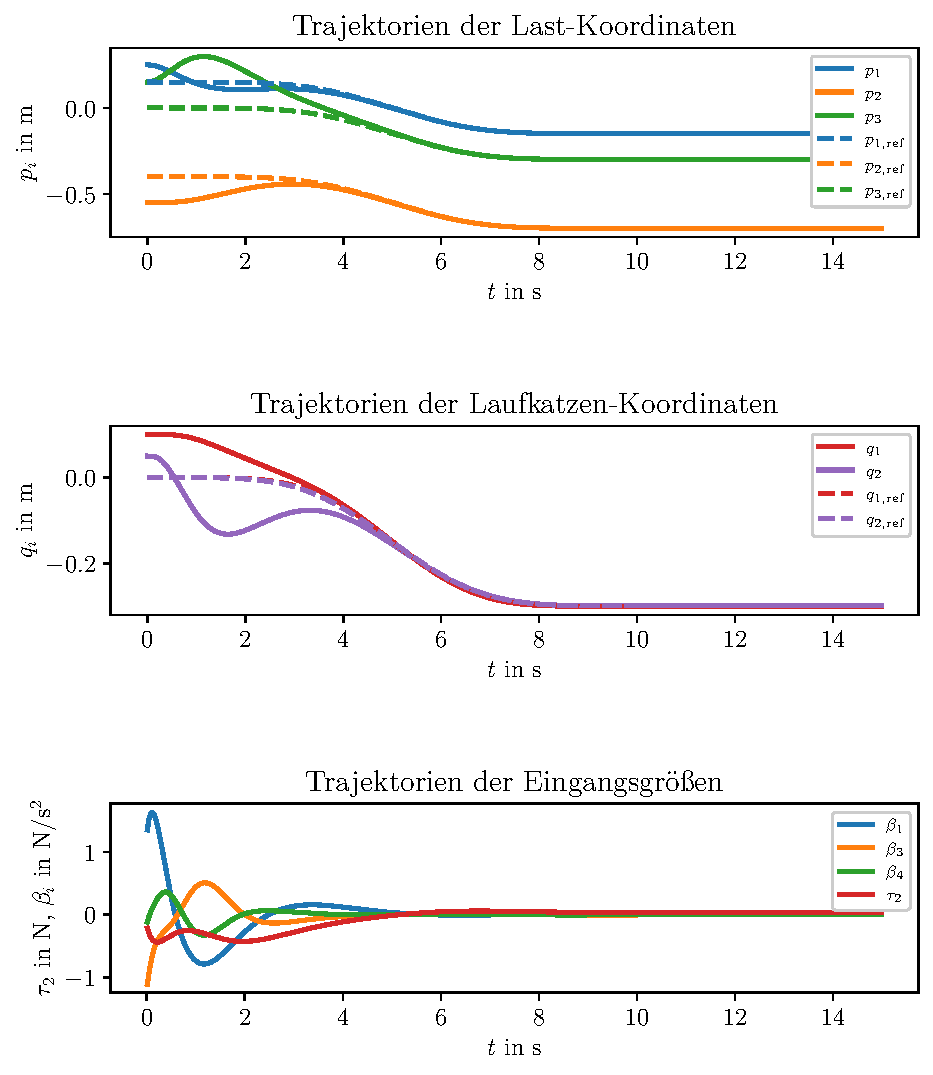
\includegraphics[scale=1]{Pictures/dyn_controller_initial_error}
	\end{center}
	\caption[Trajektorien Ruhelagenüberführung mit Regelung über dynamische Erweiterung]
	{Prototypische Trajektorien des Doppelkransystems bei der Überführung zwischen zwei Ruhelagen unter der Ausregelung von Anfangsfehlern über die dynamische Erweiterung.}
	\label{fig_dyn_controller_initial_error}
\end{figure}

\begin{figure}[H]
	\begin{center}
		% hier keine Skalierung notwendig, wenn Datei schon mit passender figsize angelegt wurde:
		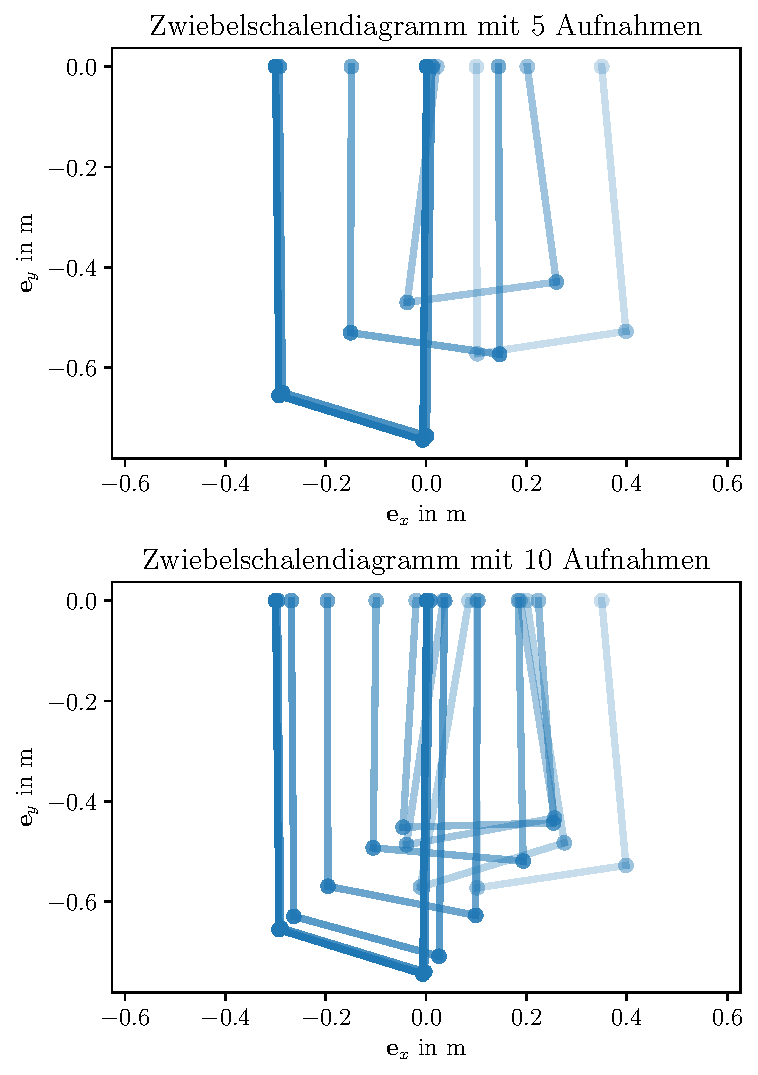
\includegraphics[scale=1]{Pictures/onion_skinned_dynamic}
	\end{center}
	\caption[Zwiebelschalendiagramm Ruhelagenüberführung mit Regelung über dynamische Erweiterung]
	{Zwiebelschalendiagramme der Bewegung der vier Gelenke sowie der beiden Seile und der Last für prototypische Trajektorien des Doppelkransystems bei der Überführung zwischen zwei Ruhelagen unter der Ausregelung von Anfangsfehlern über die dynamische Erweiterung.}
	\label{onion_skinned_dyn_controller_initial_error}
\end{figure}

\subsection{Quasi-statische Rückführungen}
\label{sec:quasi_static_control}
Eine Implementierung der in diesem Abschnitt durchgeführten Überlegungen ist unter \cite[flatness\_notebooks/ODE\_flatness\_trajectory\_control\_simulation\_qstat.ipynb]{SAGithub} zu finden.

Ebenso wie die dynamische Erweiterung kann eine quasi-statische Zustandsrückführung bei einem nicht wohldefinierten relativen vektoriellen Grad im statischen Ansatz zur Stabilisierung des Systems angesetzt werden. Dafür wird das Vorgehen nach \cite[S. 206]{NLRT_Roebenack} im Folgenden nachvollzogen und am Doppelkransystem angewendet. Tabelle \ref{tab:input_occurence} stellt für jede Eingangskomponente die Ableitungsordnung jeder Ausgangskomponente von $\mathbf{y}$ gegenüber.

\begin{table}[htbp]%
	\centering
	\caption{Auftreten der Eingänge $\tau_j$ bei Ableitungsordnung $k$ der Ausgänge $y_i$.}
	\label{tab:input_occurence}
	\begin{tabular}{ c| c c c c } 
		\toprule
		$k$ & $\tau_1$ & $\tau_2$ & $\tau_3$ & $\tau_4$ \\ 
		\hline
		$y_1^{(k)}$ & 4 & 4 & 2 & 2\\ 
		$y_2^{(k)}$ & 4 & 4 & 2 & 2\\
		$y_3^{(k)}$ & 4 & 4 & 2 & 2\\		
		$y_4^{(k)}$ & 2 & >4 & 2 & 4\\
		$(y_5^{(k)} = q_2^{(k)}$ & >4 & 2 & 4 & 2)\\
		\bottomrule
	\end{tabular}
\end{table}

Erneut wird o.B.d.A. der flache Ausgang ${\mathbf{y} = (y_1, y_2, y_3, y_4)^T = (p_1, p_2, p_3, q_1)^T}$ betrachtet. Die zeitlichen Ausgangsableitungen können wieder rekursiv gemäß Gleichung \eqref{eq:Lie_time_deriv} mittels Lie-Ableitungen bezüglich des hierfür erweiterten Zustandsvektors $\tilde{\mathbf{x}} = (\mathbf{x}, \boldsymbol{\tau}, \dot{\boldsymbol{\tau}})^T$ entlang des Vektorfelds der Zustandsgleichungen $\tilde{\boldsymbol{\delta}} = \tilde{\mathbf{f}} + \tilde{\mathbf{g}} \tilde{\boldsymbol{\tau}}$ mit
\begin{equation}
\tilde{\boldsymbol{\delta}} =
\left(\begin{matrix}
\mathbf{f} + \mathbf{g} \boldsymbol{\tau}\\
\dot{\boldsymbol{\tau}} \\
\ddot{\boldsymbol{\tau}}
\end{matrix}\right)
\end{equation}
generiert werden.

Die Eingangskomponente $\tau_3$ tritt das erste Mal bei $r_1 = 2$ in $\ddot{y}_1$ sowie auch in allen sonstigen zweiten Ableitungen des flachen Ausgangs auf. Dies gilt nicht für alle Eingangskomponenten, da der relative vektorielle Grad für $r_i = 2$ für $i = 1, ..., 4$ nicht wohldefiniert ist.

Außerdem tritt $\tau_4$ auch bei $r_3 = 2$ in $\ddot{y}_1$, $\ddot{y}_2$ und $\ddot{y}_3$, nicht aber in $\ddot{y}_4$ auf. Dies entspricht nicht der in \cite[S. 206]{NLRT_Roebenack} dargestellten Form, bei der für das Auftreten von $u_2$ der Ausgang $y_2$ noch weiter differenziert werden muss. $\tau_2$ erscheint das erste Mal explizit bei $r_i = 4$ in $y_1^{(4)}$, $y_2^{(4)}$ oder $y_3^{(4)}$, $\tau_1$ zuerst bei $r_4 = 2$ in $\ddot{y}_4$.

Eine Definition der neuen virtuellen Eingänge $v_i$ ist so möglich:
\begin{align}
\begin{split}
	\ddot{y}_1 = \ddot{p}_1 &=: v_1 = \mathrm{func}(\mathbf{x}, \tau_3, \tau_4) \\
	y_2^{(4)} = p_2^{(4)} &=: v_2 = \mathrm{func}(\mathbf{x}, \tau_1, \tau_2, \tau_3, \tau_4, \dot{\tau}_3, \dot{\tau}_4, \ddot{\tau}_3, \ddot{\tau}_4) \\
	\ddot{y}_3 = \ddot{p}_3 &=: v_3 = \mathrm{func}(\mathbf{x}, \tau_3, \tau_4) \\
	\ddot{y}_4 = \ddot{q}_1 &=: v_4 = \mathrm{func}(\mathbf{x}, \tau_1, \tau_3) .
\end{split}
\end{align}

Daraus ist ersichtlich, dass durch ein Gleichungssystem aus $v_1$, $v_3$ und $v_4$ in denen die Eingangskomponenten $\tau_1$, $\tau_3$ und $\tau_4$ affin auftreten, eine explizite Darstellung dieser Komponenten möglich ist. Dies steht im Gegensatz zur Situation in \cite[S. 207]{NLRT_Roebenack}, bei der die relativen Grade der Ausgangskomponenten aufsteigend sind, so dass kein Gleichungssystem gelöst werden muss, sondern sukzessives Einsetzen der vorher berechneten Eingänge und die algebraische Umformung der abgeleiteten Ausgänge genügt.
 
Die Berechnung von $\tau_2$ erfordert einen größeren Aufwand als bei den anderen Eingangskomponenten. Dabei ist die Substitution bisheriger Eingangskomponenten und deren Ableitungen notwendig, welche analog zu Gleichung \eqref{eq:Lie_time_deriv} aus den Lie-Ableitungen entlang $\tilde{\boldsymbol{\delta}}$ generiert werden können. Es folgt ein relativ umfangreicher Ausdruck für $\tau_2$, der zu diesem Zeitpunkt mehr als einhunderttausend Rechenoperationen enthält.

Nach \cite[S. 208]{NLRT_Roebenack} können lineare Fehlerdynamiken und daraus $\mathbf{v}$ entsprechend der jeweiligen relativen Grade der Ausgangskomponenten zur Stabilisierung des Systems angesetzt werden. Die Komponenten des virtuellen Eingangs $v_1$, $v_3$ und $v_4$ sind jeweils nur von den Zustandskomponenten $\tilde{\mathbf{x}}$ abhängig. Die Komponente $v_2$ hängt allerdings auch von den Ableitungen $\ddot{y}_2 = \ddot{p}_2$ und $y_2^{(3)} = p_2^{(3)}$ ab, welche durch Lie-Ableitungen berechnet werden können:
\begin{align}
	\label{eq:p2_derivs_Lie}
	\begin{split}
		\ddot{p}_2 &= \ddot{y}_2 = L_{\tilde{\boldsymbol{\delta}}} \dot{y}_2 = L_{\tilde{\boldsymbol{\delta}}} \dot{p}_2 \\
		p_2^{(3)} &= y_2^{(3)} = L_{\tilde{\boldsymbol{\delta}}} \ddot{p}_2.
	\end{split}
\end{align}

Außerdem werden in der Darstellung von $\tau_2$ Ableitungen der Eingangskomponenten $v_1$, $v_3$ und $v_4$ benötigt, die aus deren Fehlerdynamiken zweiter Ordnung folgen:
\begin{align}
	\begin{split}
	    \ddot{e}_i + c_{i,1} \dot{e}_i + c_{i, 0} e_i &= 0 \\
		e_i^{(3)} + c_{i, 1} \ddot{e}_i + c_{i, 0} \dot{e}_i &= 0 \\
		e_i^{(3)} + c_{i, 1} (-c_{i, 1} \dot{e}_i - c_{i, 0} e_i) + c_{i, 0} \dot{e}_i &= 0 \\
		e_i^{(3)} - c_{i, 1}^2 \dot{e}_i + c_{i, 0} \dot{e}_i - c_{i, 0} c_{i, 1} e_i &= 0 \\
		e_i^{(3)} + (c_{i, 0} - c_{i, 1}^2) \dot{e}_i - c_{i, 0} c_{i, 1} e_i &= 0 \\
		e_i^{(4)} + (c_{i, 0} - c_{i, 1}^2) \ddot{e}_i - c_{i, 0} c_{i, 1} \dot{e}_i &= 0 \\
		e_i^{(4)} + (c_{i, 0} - c_{i, 1}^2) (-c_{i, 1} \dot{e}_i - c_{i, 0} e_i) - c_{i, 0} c_{i, 1} \dot{e}_i &= 0 \\
		e_i^{(4)} + (c_{i, 1}^3 - 2 c_{i, 0} c_{i, 1}) \dot{e}_i + (c_{i, 0} c_{i, 1}^2 - c_{i, 0}^2) e_i &= 0 \\
		\Rightarrow \text{ für } i = 1,3,4: \dot{v}_i = y_i^{(3)} &= y_{i, \text{ref}}^{(3)} - (c_{i, 0} - c_{i, 1}^2) \dot{e}_i + c_{i, 0} c_{i, 1} e_i \\
		\ddot{v}_i = y_i^{(4)} &= y_{i, \text{ref}}^{(4)} - (c_{i, 1}^3 - 2 c_{i, 0} c_{i, 1}) \dot{e}_i - (c_{i, 0} c_{i, 1}^2 - c_{i, 0}^2) e_i.
	\end{split}
\end{align}

Die Komponente $v_2$ ergibt sich nach einem Ansatz vierter Ordnung unter Einbeziehung des Zusammenhangs \eqref{eq:p2_derivs_Lie}:
\begin{equation}
	v_2 = y_2^{(4)} = y_{2, \text{ref}}^{(4)} - c_{2, 3} (y_2^{(3)} - y_{2, \text{ref}}^{(3)}) - c_{2, 2} (\ddot{y}_2 - \ddot{y}_{2, \text{ref}}) - c_{2, 1} (\dot{y}_2 - \dot{y}_{2, \text{ref}}) - c_{2, 0} (y_2 - y_{2, \text{ref}})
\end{equation} 

Auf die konkrete symbolische Angabe der Stellgesetze des Systemeingangs wird aus Praktikabilitätsgründen verzichtet und stattdessen auf das zu Beginn dieses Abschnitts \ref{sec:quasi_static_control} erwähnte Jupyter-Notebook verwiesen. Übersichtlicher ist an dieser Stelle eine Angabe von funktionalen Abhängigkeiten:
\begin{subequations}
	\begin{align}
		\tau_1 &= \mathrm{func}(\mathbf{x}, \mathbf{y}_{\mathrm{ref}}, \dot{\mathbf{y}}_{\mathrm{ref}}, \ddot{\mathbf{y}}_{\mathrm{ref}}) \\
		\tau_2 &= \mathrm{func}(\mathbf{x}, \mathbf{y}_{\mathrm{ref}}, \dot{\mathbf{y}}_{\mathrm{ref}}, \ddot{\mathbf{y}}_{\mathrm{ref}}, \mathbf{y}_{\mathrm{ref}}^{(3)}, \mathbf{y}_{\mathrm{ref}}^{(4)}) \\
		\tau_3 &=\mathrm{func}(\mathbf{x}, \mathbf{y}_{\mathrm{ref}}, \dot{\mathbf{y}}_{\mathrm{ref}}, \ddot{\mathbf{y}}_{\mathrm{ref}}) \\
		\tau_4 &= \mathrm{func}(\mathbf{x}, \mathbf{y}_{\mathrm{ref}}, \dot{\mathbf{y}}_{\mathrm{ref}}, \ddot{\mathbf{y}}_{\mathrm{ref}}).
	\end{align}
\end{subequations}

Bei der simulativen Untersuchung dieses Ansatzes ergibt sich bereits im reinen Vorsteuerungsfall, also ohne Anfangsfehler oder Störungen des Systems, ein Problem mit Singularitäten in den berechneten Stellgrößen. Wenn im Stellgesetz allerdings nicht alle Zustandskomponenten $\mathbf{x}$ vorkommen, sondern nur solche, welche auch Teil des flachen Ausgangs $\mathbf{y}$ und seiner Ableitungen sind, treten keine Singularitäten auf. Eine Simulation dieses Regelungsansatzes ist daher erschwert und kann erst weiter verfolgt werden, wenn dieses Problem gelöst ist.

\subsubsection{Singularitäten in der Nähe von Ruhelagen}
In allen Eingangsgrößen treten bei diesem quasi-statischen Rückführungsentwurf in der Nähe von Ruhelagen Singularitäten auf. Diese ergeben sich aufgrund numerischer Effekte. Beim Einsetzen einer zuvor ermittelten Ruhelage entstehen Definitionslücken, sowohl Zähler als auch Nenner der Eingangsgrößen $\boldsymbol{\tau}$ werden Null. Es ist nicht auszuschließen, dass diese Lücken durch algebraische Manipulation hebbar sind. Allerdings ist eine weitere händische Untersuchung dieses Zusammenhangs mit hohem Aufwand verbunden und wird im Rahmen dieser Arbeit nicht weiter verfolgt. Die CAS-Bibliothek SymPy bietet mittels des Aufrufs \texttt{simplify} allerdings keine Lösung dieses Problems in den Eingangsgrößen.

Für eine weitere Betrachtung eignen sich die einfacheren Terme des Nenners $N_{1,3,4}$ von $\tau_1$, $\tau_3$ und $\tau_4$:
\begin{flalign}
	\begin{split}
	N_{1,3,4} &= s_{2} (- 4 l_{0} pm_{1} \sin{(pm_{3})} + 2 l_{0} pm_{2} \cos{(pm_{3})} + 4 l_{0} qm_{1} \sin{(pm_{3})} + l_{0} s_{2} \sin{(2 pm_{3})}\\
	&+ 4 pm_{1}^{2} \sin{(pm_{3})} - 4 pm_{1} pm_{2} \cos{(pm_{3})}- 4 pm_{1} qm_{1} \sin{(pm_{3})} - 4 pm_{1} qm_{2} \sin{(pm_{3})}\\
	&+ 2 pm_{2} qm_{1} \cos{(pm_{3})} + 2 pm_{2} qm_{2} \cos{(pm_{3})} + 4 qm_{1} qm_{2} \sin{(pm_{3})} - qm_{1} s_{2} \sin{(2 pm_{3})}\\
	&+ qm_{2} s_{2} \sin{(2 pm_{3})}).
	\end{split}
\end{flalign}

Des Weiteren ist die Fragestellung von Interesse, weshalb sich solche Lücken bei der Konstruktion der Trajektorie in den Ruhelagen ergeben.

\subsection{Exact feedforward linearization}
\label{sec:exact_feedforward_lin_control}
Eine Implementierung der in diesem Abschnitt durchgeführten Überlegungen ist unter \cite[flatness\_notebooks/ODE\_flatness\_trajectory\_control\_simulation.ipynb]{SAGithub} zu finden.

Bei der exact feedforward linearization wird ein Ansatz verfolgt, bei dem statt einer Kompensation der Nichtlinearität mittels Rückführung der gemessenen beziehungsweise simulierten Zustandskomponenten $\mathbf{x}$ wie bei der exakten Eingangs-Ausgangs-Linearisierung die Referenztrajektorie $\mathbf{x_{\text{ref}}}$ eingesetzt wird \cite{Hagenmeyer2003}.

Heuristisch wird eine Fehlerdynamik der Ordnung zwei für alle Komponenten des Koordinatenvektors $\boldsymbol{\theta} = (p_1, p_2, p_3, q_1, q_2)^T$ (nicht nur solchen, die auch Teil des flachen Ausgangs sind!) angesetzt:
\begin{equation}
	\ddot{\boldsymbol{\theta}} = \ddot{\boldsymbol{\theta}}_{\text{ref}} - \mathbf{c}_1^T \dot{\mathbf{e}} - \mathbf{c}_0^T \mathbf{e}.
\end{equation}

Aus der Zusammensetzung des Zustandsvektors $\mathbf{x} = (\boldsymbol{\theta}, \dot{\boldsymbol{\theta}})^T$ und der eingangsaffinen Zustandsraumdarstellung in Gleichung \eqref{eq:state_space_vector_degree} kann außerdem der Zusammenhang:
\begin{equation}
	\ddot{\boldsymbol{\theta}} = \mathbf{f}_{[6, 10]}(\boldsymbol{\theta}) + \mathbf{g}_{[6, 10]}(\boldsymbol{\theta}) \ \boldsymbol{\tau}
\end{equation}

hergestellt werden. Dabei bedeutet die Indizierung $\bullet_{[i, j]}$, die Auswahl der Zeilen $i$ bis $j$ von $\bullet$. Da für den Systemeingang $\boldsymbol{\tau} \in \mathbb{R}^4$ und für die Eingangsmatrix $\mathbf{g}_{[6, 10]} \in \mathbb{R}^{5 \times 4}$ gilt, kann dieser Zusammenhang über die Bildung einer Pseudo-Inversen $\mathbf{g}_{[6, 10]}^+$ nach dem Eingangsvektor aufgelöst werden:
\begin{equation}
	\boldsymbol{\tau}= \mathbf{g}^{+}_{[6, 10]} (\boldsymbol{\theta}) \ (\ddot{\boldsymbol{\theta}}_{\text{ref}} - \mathbf{c}_{1} \mathbf{\dot{e}} - \mathbf{c}_{0} \mathbf{e} - \mathbf{f}_{[6, 10]}(\boldsymbol{\theta})).
\end{equation}

Durch Einsetzen der Referenztrajektorien der Koordinaten $\boldsymbol{\theta}_{\text{ref}}$ in $\mathbf{g}_{[6, 10]}^+(\boldsymbol{\theta})$ und $\mathbf{f}_{[6, 10]}(\boldsymbol{\theta})$ wird die exact feedforward linearization realisiert:
\begin{equation}
\label{eq:control_law__ff_lin_pseudo}
\boldsymbol{\tau}= \mathbf{g}^{+}_{[6, 10]} (\boldsymbol{\theta}_{\text{ref}}) \ (\ddot{\boldsymbol{\theta}}_{\text{ref}} - \mathbf{c}_{1} \mathbf{\dot{e}} - \mathbf{c}_{0} \mathbf{e} - \mathbf{f}_{[6, 10]}(\boldsymbol{\theta}_{\text{ref}})).
\end{equation} 

Abbildung \ref{fig_feedforward_pseudo_controller_initial_error} zeigt prototypische Trajektorien beim Übergang zwischen zwei Ruhelagen mit einem auszuregelnden Anfangsfehler für diesen Regelungsansatz.

\begin{figure}[H]
	\begin{center}
		% hier keine Skalierung notwendig, wenn Datei schon mit passender figsize angelegt wurde:
		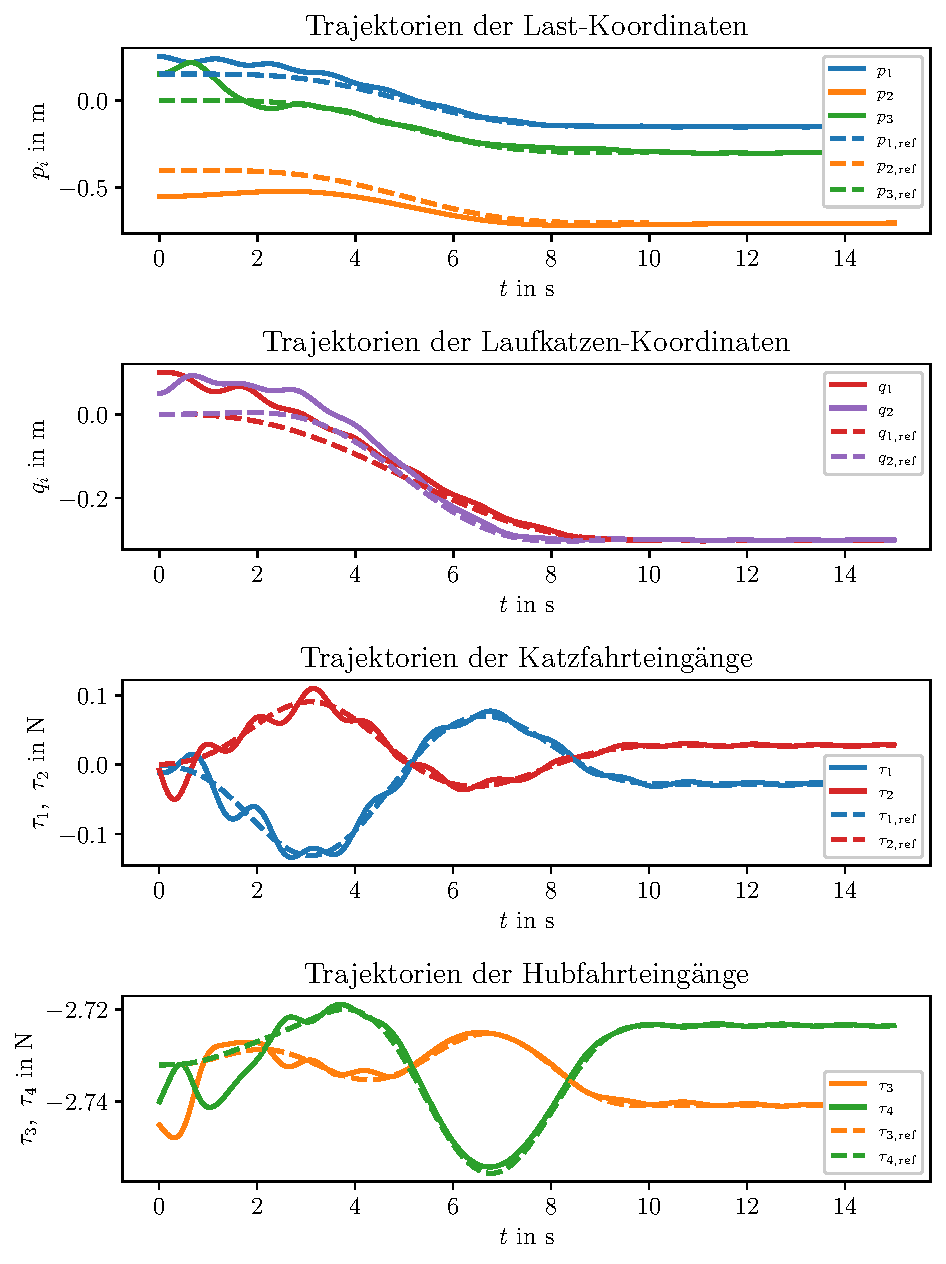
\includegraphics[scale=1]{Pictures/feedforward_lin_pseudo_controller_initial_error}
	\end{center}
	\caption[Trajektorien Ruhelagenüberführung mit Regelung über exact feedforward linearization (Pseudoinverse)]
	{Prototypische Trajektorien des Doppelkransystems bei der Überführung zwischen zwei Ruhelagen unter der Ausregelung von Anfangsfehlern über die exact feedforward linearization mit Pseudoinverser.}
	\label{fig_feedforward_pseudo_controller_initial_error}
\end{figure}

\subsubsection{Vereinfachung mittels Ausgangsselektion}
Statt der Nutzung einer Pseudo-Inversen wie in Gleichung \eqref{eq:control_law__ff_lin_pseudo} wird im Folgenden eine Selektion von vier der fünf Gleichungen der Beschleunigungen $\ddot{\boldsymbol{\theta}}$ vorgenommen. Symbolisch wird dies über eine Selektionsmatrix $\mathbf{S}$ dargestellt:
\begin{equation}
	\mathbf{S} \cdot \ddot{\boldsymbol{\theta}} = \mathbf{S} \cdot (\ddot{\boldsymbol{\theta}}_{\text{ref}} - \mathbf{c}_1^T \dot{\mathbf{e}} - \mathbf{c}_0^T \mathbf{e}) = \mathbf{S} \cdot \mathbf{f}_{[6, 10]}(\boldsymbol{\theta}) + \mathbf{S} \cdot \mathbf{g}_{[6, 10]}(\boldsymbol{\theta}) \ \boldsymbol{\tau}.
\end{equation} 

Durch die Wahl der letzten vier Gleichungen kann eine direkte Inversion der somit quadratischen Eingangsmatrix $\mathbf{g}_{[7, 10]} = \mathbf{S} \cdot \mathbf{g}_{[6, 10]}$ erfolgen:
\begin{equation}
	\boldsymbol{\tau}= \mathbf{g}^{-1}_{[7, 10]}(\boldsymbol{\theta}_{\text{ref}}) \cdot \mathbf{S} \cdot (\ddot{\boldsymbol{\theta}}_{\text{ref}} - \mathbf{c}_{1} \mathbf{\dot{e}} - \mathbf{c}_{0} \mathbf{e} - \mathbf{f}_{[6, 10]}(\boldsymbol{\theta}_{\text{ref}})) \text{ mit } 
	\mathbf{S} = 
	\begin{pmatrix}
	0 & 1 & 0 & 0 & 0 \\
	0 & 0 & 1 & 0 & 0 \\
	0 & 0 & 0 & 1 & 0 \\
	0 & 0 & 0 & 0 & 1 \\
	\end{pmatrix}.
\end{equation}

Diese Berechnungsvorschrift der Stellgrößen enthält deutlich weniger Operationen als alle zuvor dargestellten Ansätze. Damit eignet sie sich insbesondere für eine spätere Implementierung auf einem Echtzeitsystemen sowie sehr viel kürzeren Simulationszeiten. Abbildung \ref{fig_feedforward_selec_controller_initial_error} zeigt, dass sich für Beispieltrajektorien mit Anfangsfehlern ebenso wie bei den vorherigen Ansätzen ein sehr gutes Folgeverhalten sowie eine stationäre Genauigkeit ergibt.

Auf die konkrete symbolische Angabe der Stellgesetze des Systemeingangs wird aus Praktikabilitätsgründen dennoch verzichtet, da jede Eingangskomponente trotzdem mehr als einhundert Rechenoperationen beinhaltet. Stattdessen wird auf das zu Beginn dieses Abschnitts \ref{sec:exact_feedforward_lin_control} erwähnte Jupyter-Notebook verwiesen. Übersichtlicher ist an dieser Stelle eine Angabe von funktionalen Abhängigkeiten:
\begin{subequations}
	\begin{align}
		\tau_1 &= \mathrm{func}(\mathbf{x}, \boldsymbol{\theta}_{\mathrm{ref}}, \dot{\boldsymbol{\theta}}_{\mathrm{ref}}, \ddot{\boldsymbol{\theta}}_{\mathrm{ref}}) \\
		\tau_2 &= \mathrm{func}(\mathbf{x}, \boldsymbol{\theta}_{\mathrm{ref}}, \dot{\boldsymbol{\theta}}_{\mathrm{ref}}, \ddot{\boldsymbol{\theta}}_{\mathrm{ref}}) \\
		\tau_3 &= \mathrm{func}(\mathbf{x}, \boldsymbol{\theta}_{\mathrm{ref}}, \dot{\boldsymbol{\theta}}_{\mathrm{ref}}, \ddot{\boldsymbol{\theta}}_{\mathrm{ref}}) \\
		\tau_4 &= \mathrm{func}(\mathbf{x}, \boldsymbol{\theta}_{\mathrm{ref}}, \dot{\boldsymbol{\theta}}_{\mathrm{ref}}, \ddot{\boldsymbol{\theta}}_{\mathrm{ref}}).
	\end{align}
\end{subequations}

\subsubsection{Stabilitätsbetrachtung}
Im Folgenden wird die Simulation einer prototypischen Referenztrajektorie mit dem zuletzt vorgestellten Regelungsansatz betrachtet. Die Eigenwerte der Jacobimatrix $\mathbf{J}_{\dot{\mathbf{e}}}$ einer Fehlerdynamik
\begin{align}
	\mathbf{e} &:= \mathbf{x} - \mathbf{x}_{\mathrm{ref}} \Leftrightarrow \mathbf{x} = \mathbf{e} + \mathbf{x}_{\mathrm{ref}} \\
	\dot{\mathbf{e}} &= \dot{\mathbf{x}} - \dot{\mathbf{x}}_{\mathrm{ref}} = \mathbf{f}(\mathbf{e} + \mathbf{x}_{\mathrm{ref}}) + \mathbf{g}(\mathbf{e} + \mathbf{x}_{\mathrm{ref}}) \boldsymbol{\tau} - \dot{\mathbf{x}}_{\mathrm{ref}} \\
	\mathbf{J}_{\dot{\mathbf{e}}} &= \partiell{\dot{\mathbf{e}}}{\mathbf{e}}
\end{align}
sind für eine Stabilitätsbetrachtung von Interesse. Abbildung \ref{fig_feedforward_selec_controller_ljapunov1} zeigt, dass diese Eigenwerte in diesem Fall im Zeitraum von 5 $\si{s}$ bis 9 $\si{s}$ einen positiven Realteil aufweisen. Es ist möglich, dass aufgrund des bis dahin abgeklungenen Folgefehlers keine weitere Destabilisierung des Systems stattfindet, sondern eine stationäre Genauigkeit dennoch erreicht wird. Bis zum Ende der Simulationen weisen alle Eigenwerte erneut einen negativen Realteil auf. Formal kann allerdings bereits am Beispiel einer möglichen Referenztrajektorie mit Ljapunows erster (indirekter) Methode gezeigt werden, dass dieser Regelungsansatz zu einem instabilen System zu gewissen Simulationszeitpunkten führt \cite[Vorlesung 4]{NLRT_Winkler2020}. Eine andere Wahl der Rückführung (keine lineare Dynamik) könnte dieses Problem lösen.

\begin{figure}[ht]
	\begin{center}
		% hier keine Skalierung notwendig, wenn Datei schon mit passender figsize angelegt wurde:
		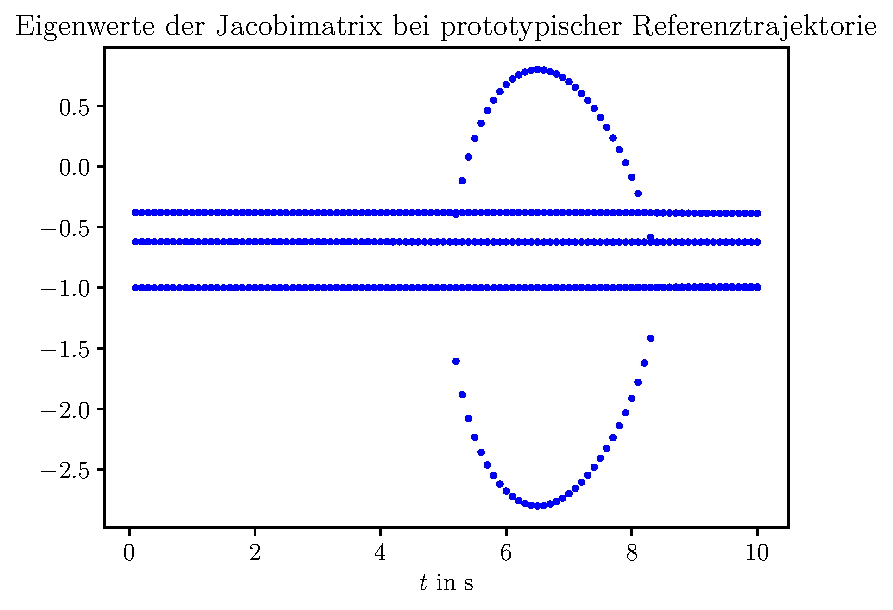
\includegraphics[scale=1]{Pictures/feedforward_lin_selec_ljapunov1}
	\end{center}
	\caption[Eigenwerte der Jacobimatrix bei Trajektorienfolge mit Regelung über exact feedforward linearization (Selektionsmatrix)]
	{Eigenwerte der Jacobimatrix $\mathbf{J}_{\dot{\mathbf{e}}}$ bei der Folge einer prototypischen Referenztrajektorie bei der Regelung über exact feedforward linearization mit Selektionsmatrix.}
	\label{fig_feedforward_selec_controller_ljapunov1}
\end{figure}

\begin{figure}[ht]
	\begin{center}
		% hier keine Skalierung notwendig, wenn Datei schon mit passender figsize angelegt wurde:
		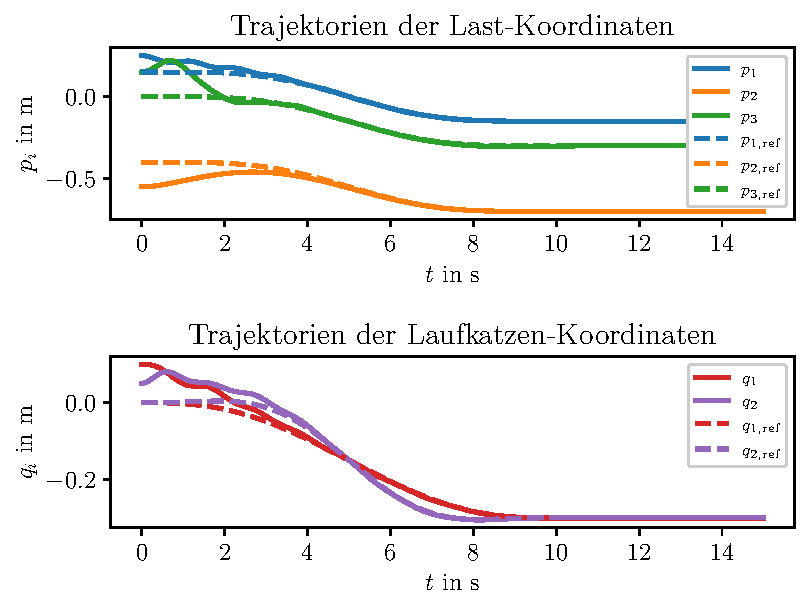
\includegraphics[scale=1]{Pictures/feedforward_lin_selec_controller_initial_error}
	\end{center}
	\caption[Trajektorien Ruhelagenüberführung mit Regelung über exact feedforward linearization (Selektionsmatrix)]
	{Prototypische Trajektorien des Doppelkransystems bei der Überführung zwischen zwei Ruhelagen unter der Ausregelung von Anfangsfehlern über die exact feedforward linearization mit Selektionsmatrix.}
	\label{fig_feedforward_selec_controller_initial_error}
\end{figure}

\chapter{Fazit und Ausblick}
\section{Fazit}
Für das zu untersuchende Brückenkransystem wurden analytische nichtlineare Modelle unter Nutzung des Lagrange-Formalismus ermittelt. Diese ergaben sich für die Lagrange-Gleichungen erster Art zu DGL- und für die Lagrange-Gleichungen zweiter Art zu DAE-Systemen. Für eine bessere Nachvollziehbarkeit der zugrunde liegenden Methodik wurde dieses Vorgehen zunächst anhand eines Einzelkransystems durchgeführt. Es erfolgte eine Identifikation aller zumeist geometrischen Modellparameter.

Die DGL-Modelle von Einzel- und Doppelkransystem wurden auf differenzielle Flachheit untersucht. Dabei wurde eine systematische Vorgehensweise für Mehrgrößensysteme skizziert. Dieses konnte auf Gleichungsebene anhand des Einzelkransystems veranschaulicht werden. Für das Doppelkransystem wurde aus Praktikabilitätsgründen auf eine explizite Darstellung der umfangreichen Ausdrücke in den Ergebnissen verzichtet. Unter Zuhilfenahme von Computeralgebrasystemen war eine Beschreibung dieser Zusammenhänge sowie Darstellung funktionaler Abhängigkeiten möglich.

Auf Grundlage des für das Doppelkransystem bestimmten flachen Ausgangs konnten polynombasierte Trajektorien der Ausgangskomponenten aufgestellt werden. Diese dienen der Überführung des Systems von einer gegebenen Ruhelage in eine andere. Auf Basis der Parametrisierung der Eingangskomponenten durch den flachen Ausgang war es möglich daraus Stellgrößenverläufe für eine Vorsteuerung abzuleiten. Zur Folgeregelung ist eine statische Rückführung aufgrund eines nicht wohldefinierten vektoriellen relativen Grades nicht möglich. Stattdessen konnte durch eine dynamische Rückführung mit linearen Fehlerdynamiken eine Stabilisierung des Systems bei Anfangsfehlern sowie Einschwingen entlang der Solltrajektorie erzielt werden, allerdings in Verbindung mit einem hohen Komplexitätsgrad des Stellgesetzes. Der Ansatz einer quasi-statischen Rückführung mündete in numerischen Problemen aufgrund von Singularitäten in der Nähe von Ruhelagen, welche im Rahmen dieser Arbeit nicht behoben wurden. Mittels der exact feedforward linearization wurde alternativ ein Regelungsansatz verfolgt, aus welchem ein kompaktes Stellgesetz folgt. Dafür wurde eine kleinere Ordnung der linearen Fehlerdynamiken angenommen sowie alle Komponenten oder auch eine heuristische Selektion der Zustandskomponenten mit diesen Fehlerdynamiken behaftet. Dieser Ansatz eignete sich während praktischer Untersuchungen ebenso zur Stabilisierung des Systems bei Anfangsfehlern, verstößt aber gegen formale Stabilitätsbedingungen.

Die Durchführung umfangreicher symbolischer Berechnungen wie auch die numerisch simulative Verfikation der ermittelten Steurungs- und Regelungsgesetze erfolgte über Jupyter-Notebooks in Python. Über eine Robustheit der Regelungsansätze wurde keine Aussage getroffen. Gerade bei nichtlinearen Systemen wie dem in dieser Arbeit untersuchten können bereits geringe Modellabweichungen zur Instabilität bei Regelungsansätzen der exakten Linearisierung führen, woraus hohe Genauigkeitsanforderungen für die Modellbildung folgen.

\section{Ausblick}

Für die Untersuchung der Eignung der ermittelten Regelungsansätze am realen Demonstratorsystem ist eine Implementierung dieser auf der vorhandenen Hardware der Raspberry Pis notwendig. Gerade die Einhaltung von Anforderungen an die Echtzeitfähigkeit bei numerisch umfangreichen Stellgesetzen stellt dabei eine Herausforderung dar.

Die flachheitsbasierte Vorsteuerung kann zuerst allein erprobt werden, so dass auch aus Betrachtung der Abweichung von Ist- und Referenztrajektorien auf die Größenordnung der Modellabweichungen geschlossen werden kann. Die Regelungsansätze sollten daraufhin unter Begrenzung von Stellgrößen und Überwachung des gegebenenfalls instabil werdenden Systems getestet werden.

Neben einer vertieften Auseinandersetzung mit der quasi-statischen Rückführung, bei der Singularitäten in den Stellgesetzen gegebenenfalls durch die Hebung von Definitionslücken vermieden werden können, verspricht auch die Nutzung moderner Regelungsansätze aus dem Gebiet des maschinellen Lernens kompaktere sowie robuste Lösungen. Über das sogenannte bestärkende Lernen (englisch reinforcement learning) können sich Agenten für den Übergang zwischen Ruhelagen selbstständig eine Strategie aneignen. Ein Transferlernen aus Stelltrajektorien klassischer Regelungsansätze auf die Agenten wäre zudem denkbar.

Eine Präzisierung des physikalischen Modells durch Einbeziehung von Reibungseffekten könnte vor allem die Effektivität der daraus abgeleiteten Vorsteuerung weiter verbessern. Allerdings ergibt bereits das einfachere aktuelle Modell bei einem flachheitsbasiertem Vorgehen äußerst umfangreiche Terme für die Stellgrößen, so dass die Anpassung zuvor darauf trainierter Agenten über beispielsweise bestärkendes Lernen eine kompaktere Lösung ergeben könnte.


%%% Local Variables:
%%% mode: latex
%%% TeX-master: "ArbeitRST"
%%% End:
